\documentclass{ltjsarticle}

\usepackage{luatexja}
\usepackage{graphicx}
\usepackage[colorlinks=true,linkcolor=blue,citecolor=blue,urlcolor=blue]{hyperref}
\usepackage{xcolor}
\usepackage{mathtools}
\usepackage{siunitx}
\usepackage{amsmath}
\usepackage{amssymb}
\usepackage{sepnum} % sepnumパッケージを読み込む
\usepackage{at}
\usepackage{bm}
\usepackage{cancel}
\usepackage{float} % ← プリアンブルに追加
\usepackage{titlesec}
\usepackage{enumitem}
\numberwithin{equation}{section} % 数式番号をセクションごとに分ける
\titleformat{\subsubsection}
  {\normalfont\large\bfseries}
  {\thesubsubsection}{1em}{}

\newcommand{\underlab}[3][.35ex]{%
  \mathrel{\mathop{#2}\limits_{\mathclap{\lower#1\hbox{\text{\footnotesize\textcircled{\scriptsize #3}}}}}}%
}

\newcommand{\ctext}[1]{\raise0.2ex\hbox{\textcircled{\scriptsize{#1}}}}

\usepackage[normalem]{ulem} % \uline, \uwave

% 直線 → \ulineunder、波線 → \uwaveunder
\newcommand{\ulineunder}[2]{%
  \underset{\smash{\text{\scriptsize #2}}}{\uline{\ensuremath{#1}}}%
}
\newcommand{\uwaveunder}[2]{%
  \underset{\smash{\text{\scriptsize #2}}}{\uwave{\ensuremath{#1}}}%
}

% 下線の“下げ量”と太さ（グローバル設定）
\setlength{\ULdepth}{1.2ex} 
\renewcommand\ULthickness{0.8pt} % 波線/直線の太さ


\usepackage[most]{tcolorbox}
\newtcolorbox{eqbox}[1]{%
  enhanced,
  colback=white, colframe=black,
  boxrule=0.4pt, arc=6pt,
  left=8pt, right=8pt, top=8pt, bottom=8pt, % 余白
  title={#1},                 % ← 引数がタイトルになる
  fonttitle=\bfseries,        % タイトルの体裁
  coltitle=black,
  colbacktitle=gray!10,       % タイトル帯の背景色（要らなければ white）
  attach boxed title to top left={yshift=-2mm, xshift=6pt}, % 箱内の左上に配置
  boxed title style={sharp corners, boxrule=0pt}, % タイトル枠線なし
}
\numberwithin{equation}{section}
\renewcommand{\thesection}{\arabic{section}}


\title{課題1：「プラズマ物理入門」}
\author{中 陽太}
\date{\today}

\begin{document}

\maketitle
\setcounter{section}{1}
\section*{(1)}
\addcontentsline{toc}{section}{(1)}

\subsection*{導出}
荷電粒子の位置$x=0$のポテンシャルを$\phi _0$として，そこから減少し，無限遠で0になるポテンシャルを考える．このときの$\phi (x)$を求める．

まず，一次元のポアソン方程式より，

\begin{equation}
  \nabla^2 \phi = \frac{d^2\phi}{dx^2} = -4\pi e(n_i - n_e) \hspace{1pc}  (Z=1) \label{1.12}
\end{equation}

電子と比べイオンの質量ははるかに重いので，イオンは運動せず，電子に対し，正電荷の一様なバックグラウンドとなっていると仮定する．もし遠方の密度が$n_\infty$ であるなら
\begin{center}
  $n_i = n_\infty$
\end{center}
となる．

ポテンシャルエネルギー$q\phi$の存在下において，電子の分布関数（ボルツマン分布）は
\[
  f(u) = A\exp\left[-\left(\frac{1}{2}mv^2 + q\phi\right)/k_BT_e\right]
\]
$q=-e$として，$u$で積分すると

\begin{align*}
  n_e &= \iiint A\exp\left[-\left(\frac{1}{2}mv^2 - e\phi\right)/k_BT_e\right]dv^3 = \underline{A}e^{\frac{e\phi}{k_B T_e}} 
\underset{\equiv n_0}{\underline{\iiint e^{-\frac{m v^2}{2 k_BT_e}} \, dv^3}}\\
       &= n_0 \exp(e\phi/KT_e)
\end{align*}
遠方（$x\to \infty$）で$\phi \to 0$より
\[
  n_e = n_0\cdot 1 = n_o = n_\infty
\]
これより

\[
 n_e =  n_\infty \exp(e\phi/k_BT_e)
\]
これを用いて式\eqref{1.12}を書き直すと

\[
  \frac{d^2\phi}{dx^2}= 4\pi en_\infty\left\{\left[\exp{\left(\frac{e\phi}{k_BT_e}\right)}\right]-1\right\}
\]
クーロンポテンシャルよりも運動エネルギーの方がはるかに大きい領域，つまり$|e\phi / k_BT_e| \ll 1$の領域においてTaylor展開することで
\begin{equation}
  \frac{d^2\phi}{dx^2} = 4\pi en_\infty\left[\frac{e\phi}{k_BT_e}+ \frac{1}{2}\left(\frac{e\phi}{k_BT_e}\right)^2 + \cdots \right] \label{1.13}
\end{equation}
となる．1次の項だけを考えると

\begin{equation}
  \frac{d^2 \phi}{dx^2} = \frac{4\pi n_\infty e^2}{k_B T_e}\phi \label{1.14}
\end{equation}
を得る．デバイ長は次のように定義される：

\begin{eqbox}{デバイ長}
\begin{equation}
 \lambda_D = \left(\frac{k_BT_e}{4\pi ne^2}\right)^{1/2} \label{1.15}
\end{equation}
\end{eqbox}
これにより，式\eqref{1.14}の解は
\begin{equation}
  \phi = \phi_0 \exp(-|x|/\lambda_D) \label{1.16}
\end{equation}
となる．式\eqref{1.16}の表す意味は，試験電荷などといった外乱で生じた静電ポテンシャルが距離とともに指数関数的に減衰し，その減衰の速さを決める長さがデバイ長 
$\lambda_D$ということである．ゆえに，デバイ長は遮蔽の距離を決める尺度となる．

\begin{figure}[H]
  \centering
  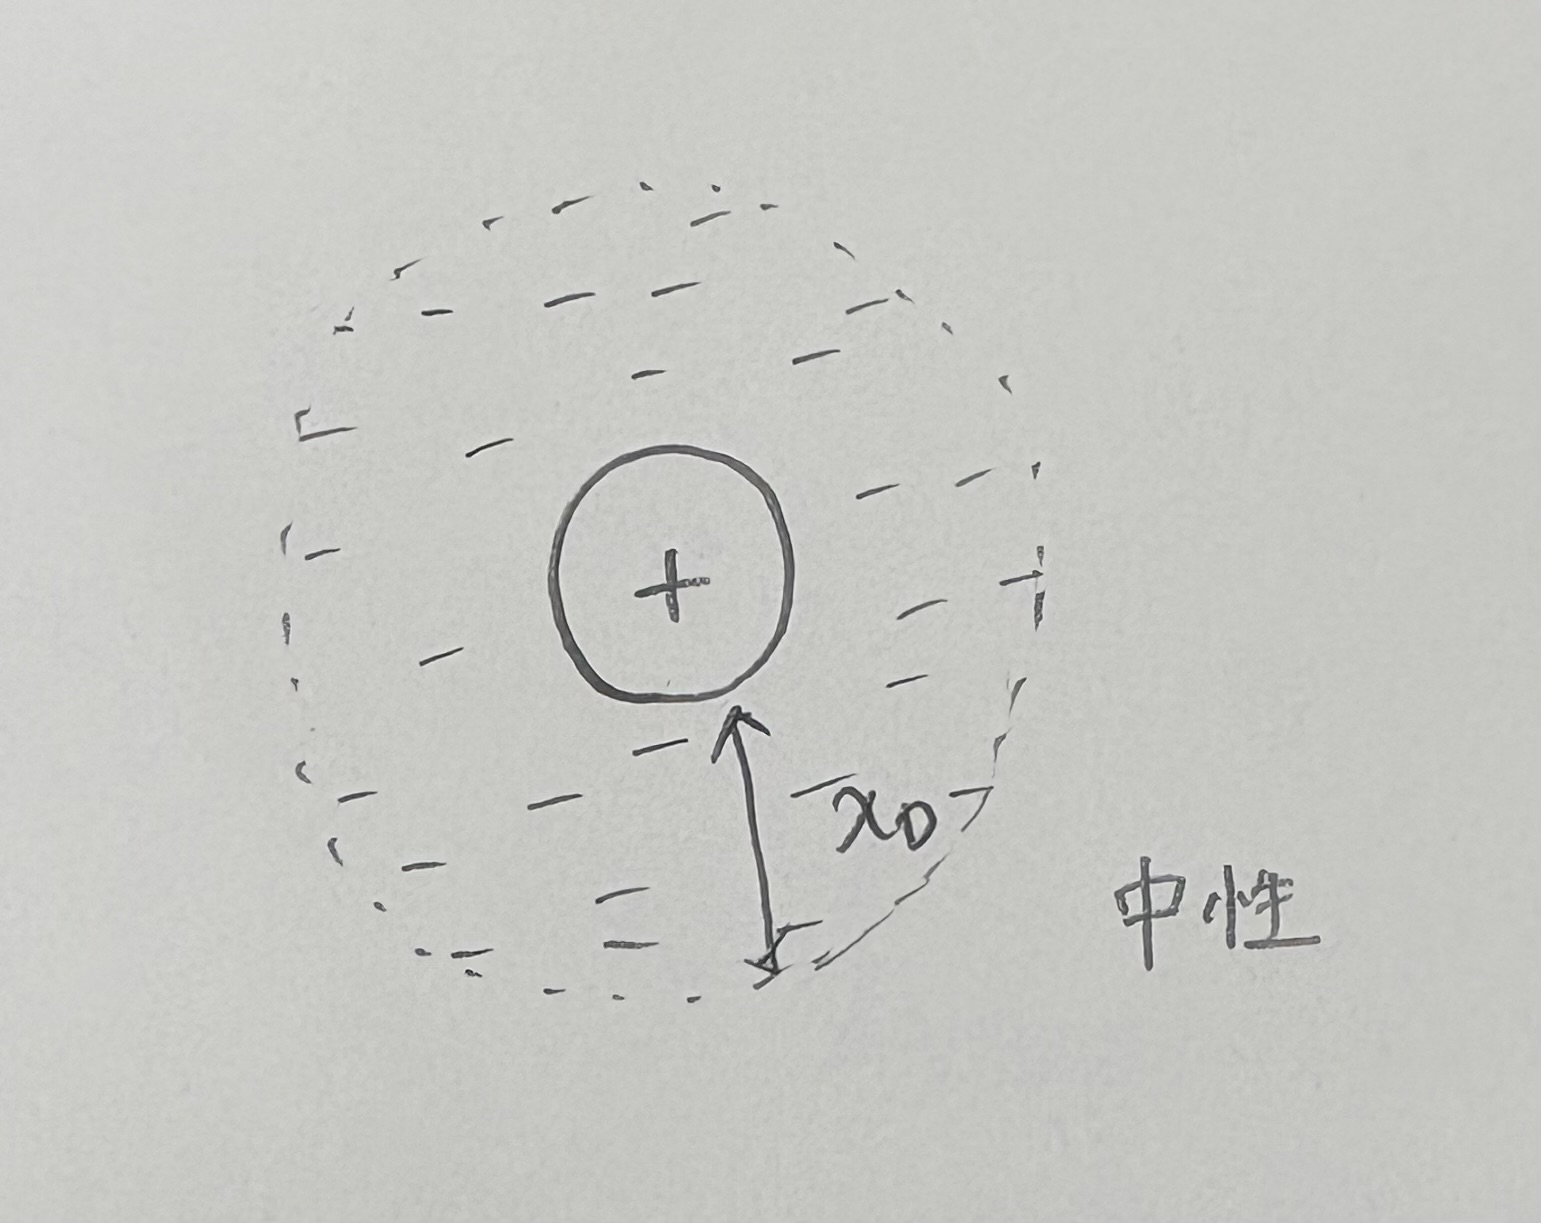
\includegraphics[width=0.4\linewidth]{assi_fig1.jpeg}
  \caption{デバイ遮蔽の様子}
\end{figure}


\setcounter{section}{2}
\section*{(2)}
\addcontentsline{toc}{section}{(2)}
\subsection{電場}
一様な電場がある場合を考える．$\bm{B}$の方向にz軸をとり，$E_y=0$となるように$\bm{E}$をx-z面に配置するように座標空間をとる．
運動方程式は

\begin{equation}
  m\frac{d\bm{v}}{dt} = q(\bm{E} + \bm{v}\times \bm{B}) \label{2.8}
\end{equation}
z成分は簡単に求まり，

\begin{equation}
  \frac{dv_z}{dt} = \frac{q}{m}E_z \hspace{3pc} \therefore v_z = \frac{qE_z}{m}t + v_{z0}
\end{equation}
となる．

残りの成分，つまり\bm{B}に垂直な面での運動は式\eqref{2.8}から
\begin{align}
  \begin{split}
    \frac{dv_x}{dt} &= \frac{q}{m}E_x \pm \omega_c v_y\\
    \frac{dv_y}{dt} &= 0 \mp \omega_c v_x
  \end{split} \label{2.10}
\end{align}
ここで，$\omega_c \equiv \frac{|q|B}{m}$はサイクロトロン周波数である．
これを微分してそれぞれ計算すると、

\begin{subequations}
  \begin{align}
    \ddot{v}_x &= -\omega_c^2v_x\\
    \ddot{v}_y &= \mp \omega_c\left(\frac{q}{m}E_x \pm \omega_c v_y\right) = -\omega^2_c v_y -\omega^2_c\frac{E_x}{B} \label{v_e.eq}
  \end{align} \label{base_eq}
\end{subequations} 
ここで，粒子がサイクロトロン運動をすることを見越して

\begin{equation}
  v_y = \uwaveunder{\pm v_\perp e^{i\omega_c t}}{サイクロトロン運動}+v_E \label{if.ve}
\end{equation}
を仮定する．これの2階微分は

\begin{equation}
  \begin{aligned}
    \ddot{v}_y = \mp \omega_c ^2 v_\perp e^{i\omega_c t} &= -\omega_c ^2 (\ulineunder{\pm v_\perp e^{i\omega_c t}+v_E}{$=\,v_y$})+\omega_c ^2 v_E\\
                                                          &= -\omega_c ^2(-v_E + v_y)
  \end{aligned}
\end{equation}
これと式\eqref{v_e.eq}を比較すると

\begin{equation}
  v_E = -\frac{E_x}{B}
\end{equation}
となる．これより，式\eqref{if.ve}を書き直すと
\begin{equation}
  v_y = \pm v_\perp e^{i\omega_c t} - \frac{E_x}{B}
\end{equation}
さらに，式\eqref{2.10}から
\begin{equation}
  v_x = \mp \frac{1}{\omega_c}\dot{v_y} = v_\perp e^{i\omega_c t}
\end{equation}
これらから，サイクロトロン運動に加えて，案内中心のy方向へのドリフト$v_E$が重ね合わされることがわかる．
$v_E$の一般式はベクトル形式で表すことができる．

\[
  \bm{E} \times \bm{B} = 
\begin{pmatrix}
E_x \\ 0 \\ E_z
\end{pmatrix}
\times
\begin{pmatrix}
0 \\ 0 \\ B
\end{pmatrix}
=
\begin{pmatrix}
0 \\ -BE_x \\ 0
\end{pmatrix}
\]
となることから

\begin{equation}
  \boxed{\bm{v}_E = \frac{\bm{E}\times \bm{B}}{B^2}} \label{general.ve}
\end{equation}
と表せる．この$\bm{v}_E$は\textcolor{red}{$\bm{E}\times \bm{B}$ドリフト}と呼ばれる．

このドリフトが生じる背景は次のように理解できる．半回転する間において，粒子は電場$E_x$により加速され，$r_L$が大きくなる．反対に，もう半回転する間は$r_L$は小さくなる。
この差が$-y$方向へのドリフトを生じさせるのである．

\begin{figure}[H]
  \centering
  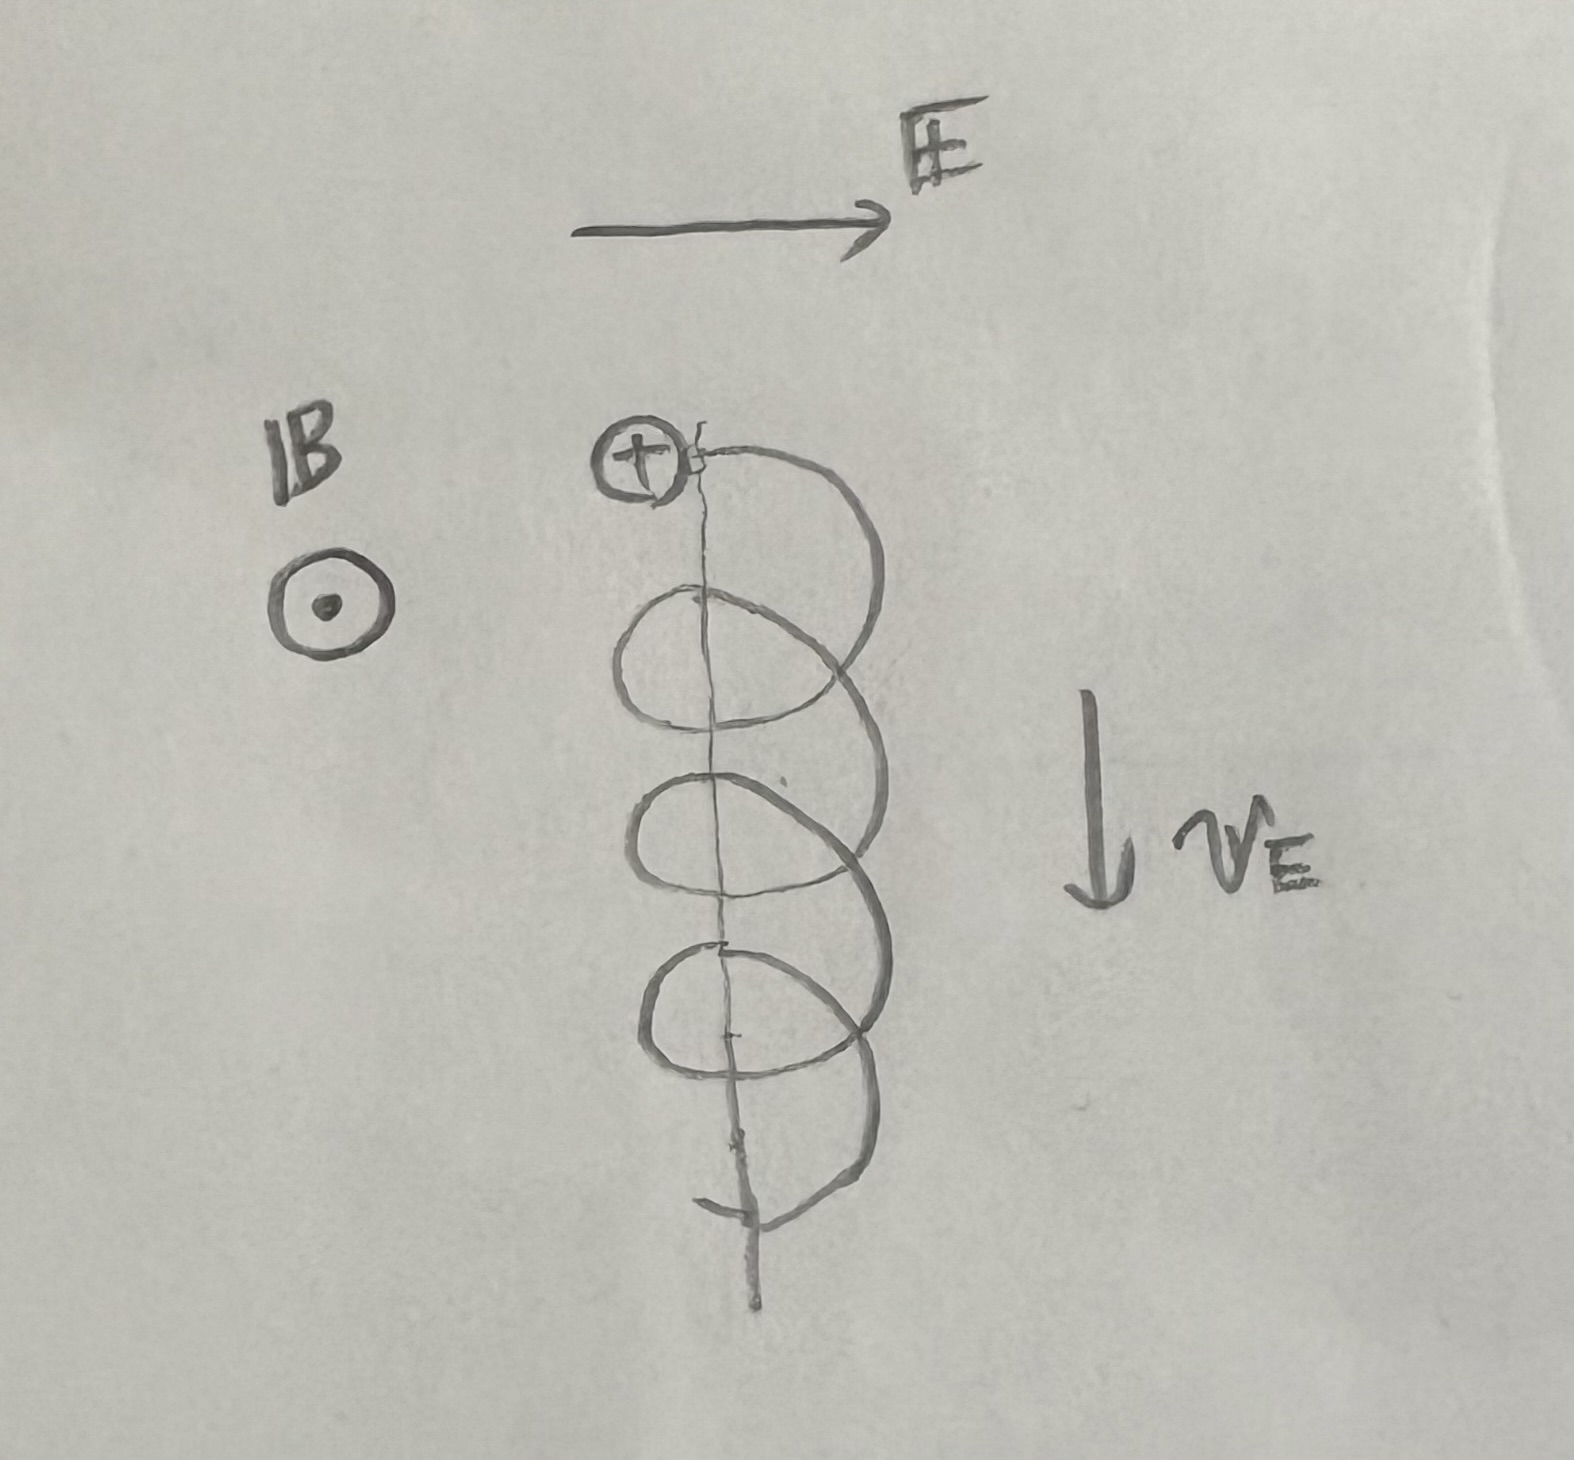
\includegraphics[width=0.5\linewidth]{figg2.jpeg}
  \caption{\bm{E}\times \bm{B}ドリフトの様子}
  \label{figg_2}
\end{figure}


\subsection{一般的な力}
先の結果は$q\bm{E} \to \bm{F}$と置き換えることで一般的な力$\bm{F}$に適用できる．$\bm{F}$による旋回中心のドリフトは\eqref{general.ve}式より

\begin{equation}
  \boxed{\bm{v}_f = \frac{1}{q}\frac{\bm{F}\times \bm{B}}{B^2}} \label{drift_F}
\end{equation}
となる．これの物理的背景は$\bm{E}\times \bm{B}$ドリフトと同じである．ただし，$\bm{v_E}$では粒子によらず同じ方向であったが，$\bm{v_f}$ではイオンと電子で方向が逆になる．
プラズマ中で電子とイオンが逆向きに動くことは電流を流れることを意味する．

\begin{figure}[H]
  \centering
  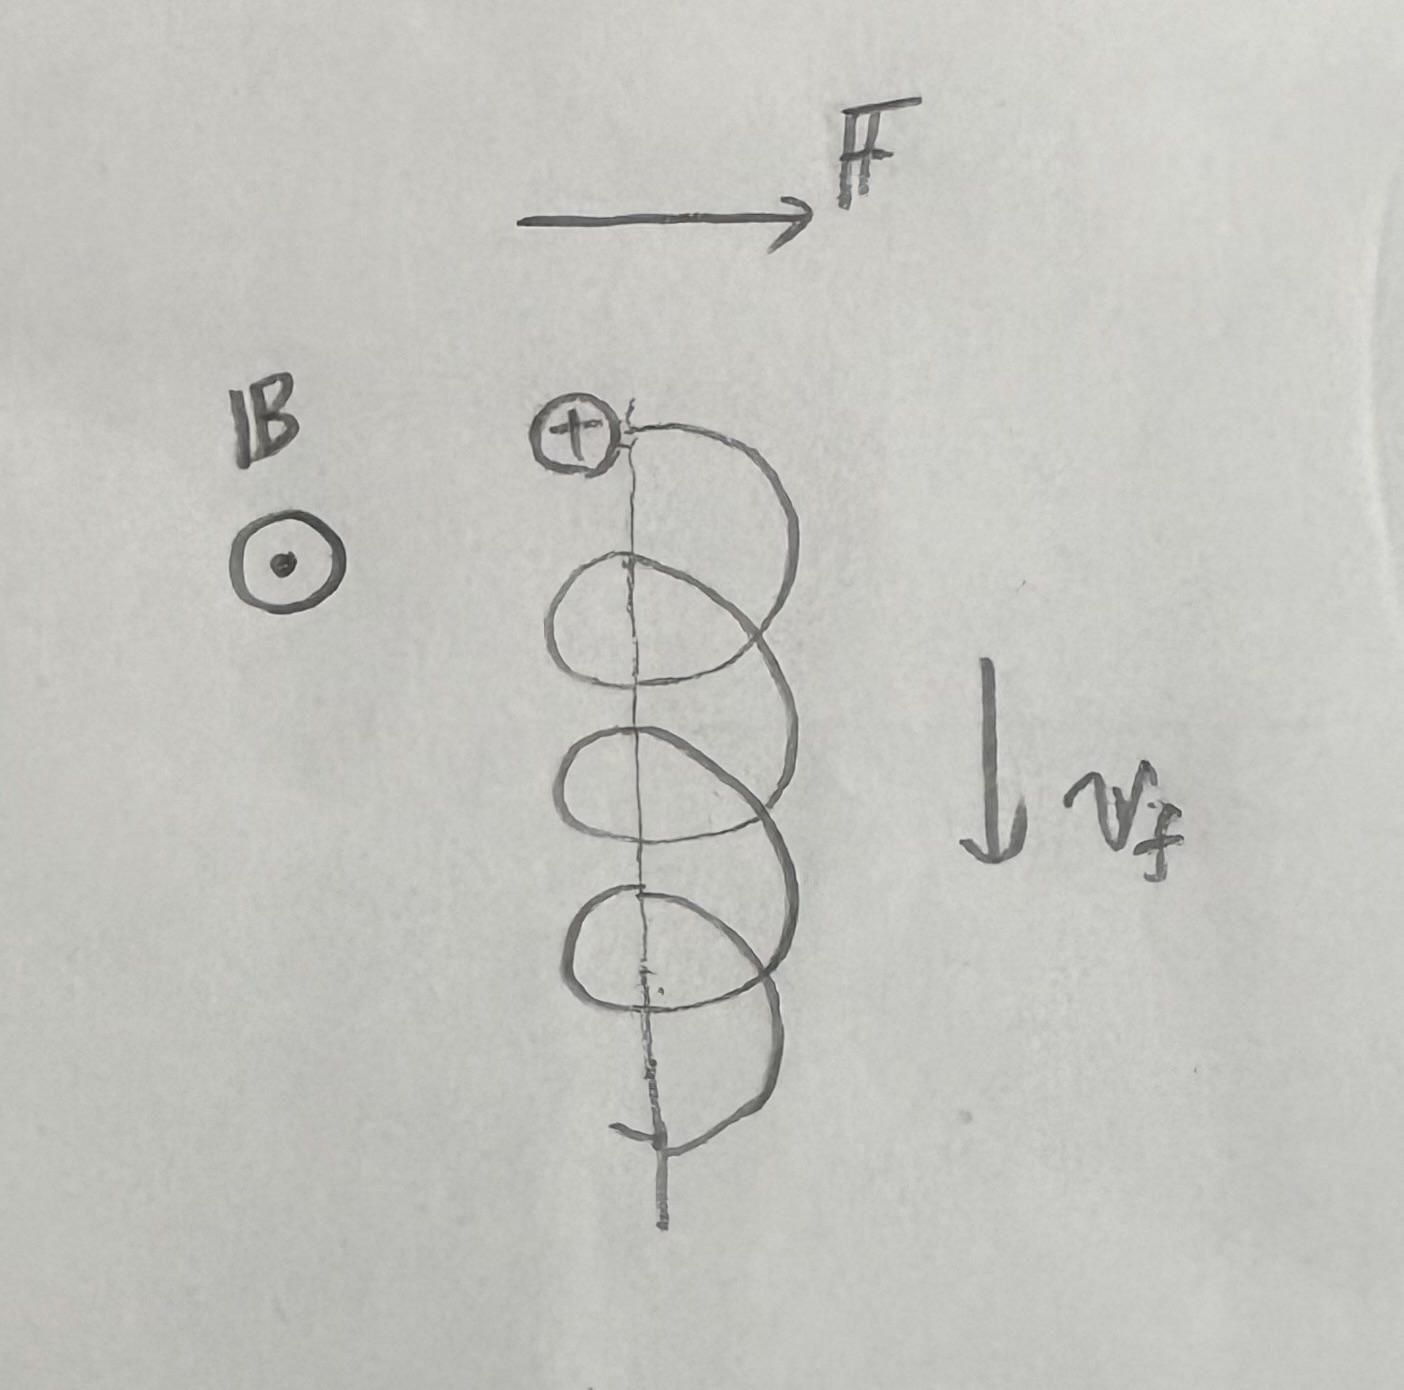
\includegraphics[width=0.5\linewidth]{figg3.jpeg}
  \caption{一般的な力$\bm{F}$を受けた時のドリフトの軌道}
  \label{figg_3}
\end{figure}

\subsection{重力場}
特に$\bm{F}$が重力$m\bm{g}$の場合には

\begin{equation}
  \boxed{\bm{v}_g = \frac{m}{q}\frac{\bm{g}\times \bm{B}}{B^2}}
\end{equation}
となる．実際には，地上の重力$\bm{g}$は小さいため，$|\bm{v}_g|$は通常，無視してよい．しかし，磁力線が曲がっている場合，後述するように遠心力に起因する「有効重力」が生じる．
遠心力は「重力」不安定と呼ばれるプラズマ不安定性の基盤である．


\subsection{非一様電場}
磁場は一様であるが，電場は非一様であるような場を考える．簡単のため，$\bm{E}$はx方向を向き，y方向に正弦状に変化すると仮定する：

\begin{equation}
  \bm{E} \equiv E_0(\cos ky)\hat{\bm{x}} \label{2.47}
\end{equation}

運動方程式は

 \begin{equation}
  m(d\bm{v}/dt) = q[\bm{E}(x) + \bm{v} \times \bm{B}] \label{2.48} 
 \end{equation}
となる．電場に垂直な成分は

\begin{equation}
  \dot{v}_x = \frac{qB}{m}v_y + \frac{q}{m}E_x(x) \hspace{2pc} \dot{v}_y = -\frac{qB}{m}v_x \label{2.49}
\end{equation}
\begin{equation}
  \ddot{v}_x = -\omega_c ^2 v_x \pm \omega_c \frac{\dot{E}_x}{B} \label{2.50}
\end{equation}
\begin{equation}
  \ddot{v}_y = -\omega_c ^2 v_y - \omega_c ^2 \frac{E_x(x)}{B} \label{2.51}
\end{equation}
これを解くために，もし電場が弱ければ，近似として，擾乱されていない軌道を$E_x(y)$の評価に使用できる．電場が存在しない場合の軌道は通常のサイクロトロン運動であり，次式で与えられる：

\begin{equation}
  y = y_0 \pm r_L \cos{\omega_c t} \label{2.52}
\end{equation}
式\eqref{2.51}，\eqref{2.47}より

\begin{equation}
  \ddot{v}_y = -\omega_c ^2 v_y - \omega_c ^2 \frac{E_0}{B} \cos k(y_0 \pm r_L \cos{\omega_c t}) \label{2.53}
\end{equation}
このときの$v_y$は周波数$\omega_c$で起こる高速なサイクロトロン運動とゆっくりとしたドリフト運動の2つが含まれていると予想できる．我々の目標はドリフト速度$v_E$を求めることであるから，
サイクロトロン運動の振動成分を除去したい．そのため，1サイクルで平均を取る．

まず，$\bar{v}_x$について式\eqref{2.50}において平均をとることで，$\overline{\ddot{v}}_x = 0$，$\bar{\dot{E}}_x = 0$から$\bar{v}_x = 0$がいえる．
$\overline{\ddot{v}}_x = 0$としたことに疑問に思うかもしれない．確かに，$v_x$はサイクロトロン運動に加えて，ドリフト運動にあたる速度を持つ．しかし，時間変化を考えたとき，ドリフト運動はサイクロトロン運動に比べて極めてゆっくりであるから無視できる．
それゆえ$\overline{\ddot{v}}_x$はサイクロトロン運動のみを考えてよく，もちろんその1サイクルの平均は0になる．同様に，$\overline{\ddot{v}}_y = 0$であるから，
式\eqref{2.53}において平均をとると

\begin{equation}
  \overline{\ddot{v}}_y = 0 = -\omega_c ^2 \bar{v}_y - \omega_c^2\frac{E_0}{B}\overline{\cos k(y_0 + r_L \sin \omega_c t)} \label{2.54}
\end{equation}
Larmor半径は小さいので，$kr_L \ll 1$より$\cos$及び$\sin$についてTaylor展開すると

\begin{align}
  \cos k(y_0 +r_L \sin \omega_c t) &= \cos (ky_0) \cos (kr_L \sin \omega_c t) - \sin (ky_0) \sin (kr_L \sin \omega_c t) \notag \\ 
                                   &\approx (\cos ky_0)(1-\frac{1}{2} k^2 r_L^2 \sin^2 \omega_c t) - (\sin ky_0)kr_L \sin \omega_c t
\end{align}
これに時間平均をとれば，最後の項は消えることから．式\eqref{2.54}より

\begin{equation}
  \bar{v}_y = -\frac{E_0}{B}(\cos ky_0)\left(1-\frac{1}{4}k^2r_L ^2\right) = -\frac{E_x(y_0)}{B}\left(1-\frac{1}{4}k^2 r_L ^2\right) \label{2.57}
\end{equation}
したがって，通常の$\bm{E} \times \bm{B}$ドリフトは不均一性によって修正され，次のように表される：

 \begin{equation}
  \bm{v}_E = \frac{\bm{E} \times \bm{B}}{B^2}\left(1-\frac{1}{4}k^2r_L^2\right) \label{2.58}
 \end{equation}

正弦波分布の仮定から離れて，任意の$\bm{E}$の変動に対しては，$ik$を$\nabla$で置き換えるだけでよく，式\eqref{2.58}は次のように書ける：

\begin{equation}
  \boxed{\bm{v}_E = \left(1+\frac{1}{4}r_L^2\nabla^2\right)\frac{\bm{E}\times \bm{B}}{B^2}} \label{2.59}
\end{equation}

これは一様電場の$\bm{E}\times \bm{B}$ドリフトに空間変化分の補正項がついた形となっている．
線形に変化する電場中では，イオンは軌道の片側でより強い電場中におり，反対側では同量だけ弱い電場中にある．この場合，平均をとった際に$v_E$への補正項は打ち消し合う．ここから補正項が$E$の2階微分関数に依存することが明らかである．

\begin{figure}[H]
  \centering
  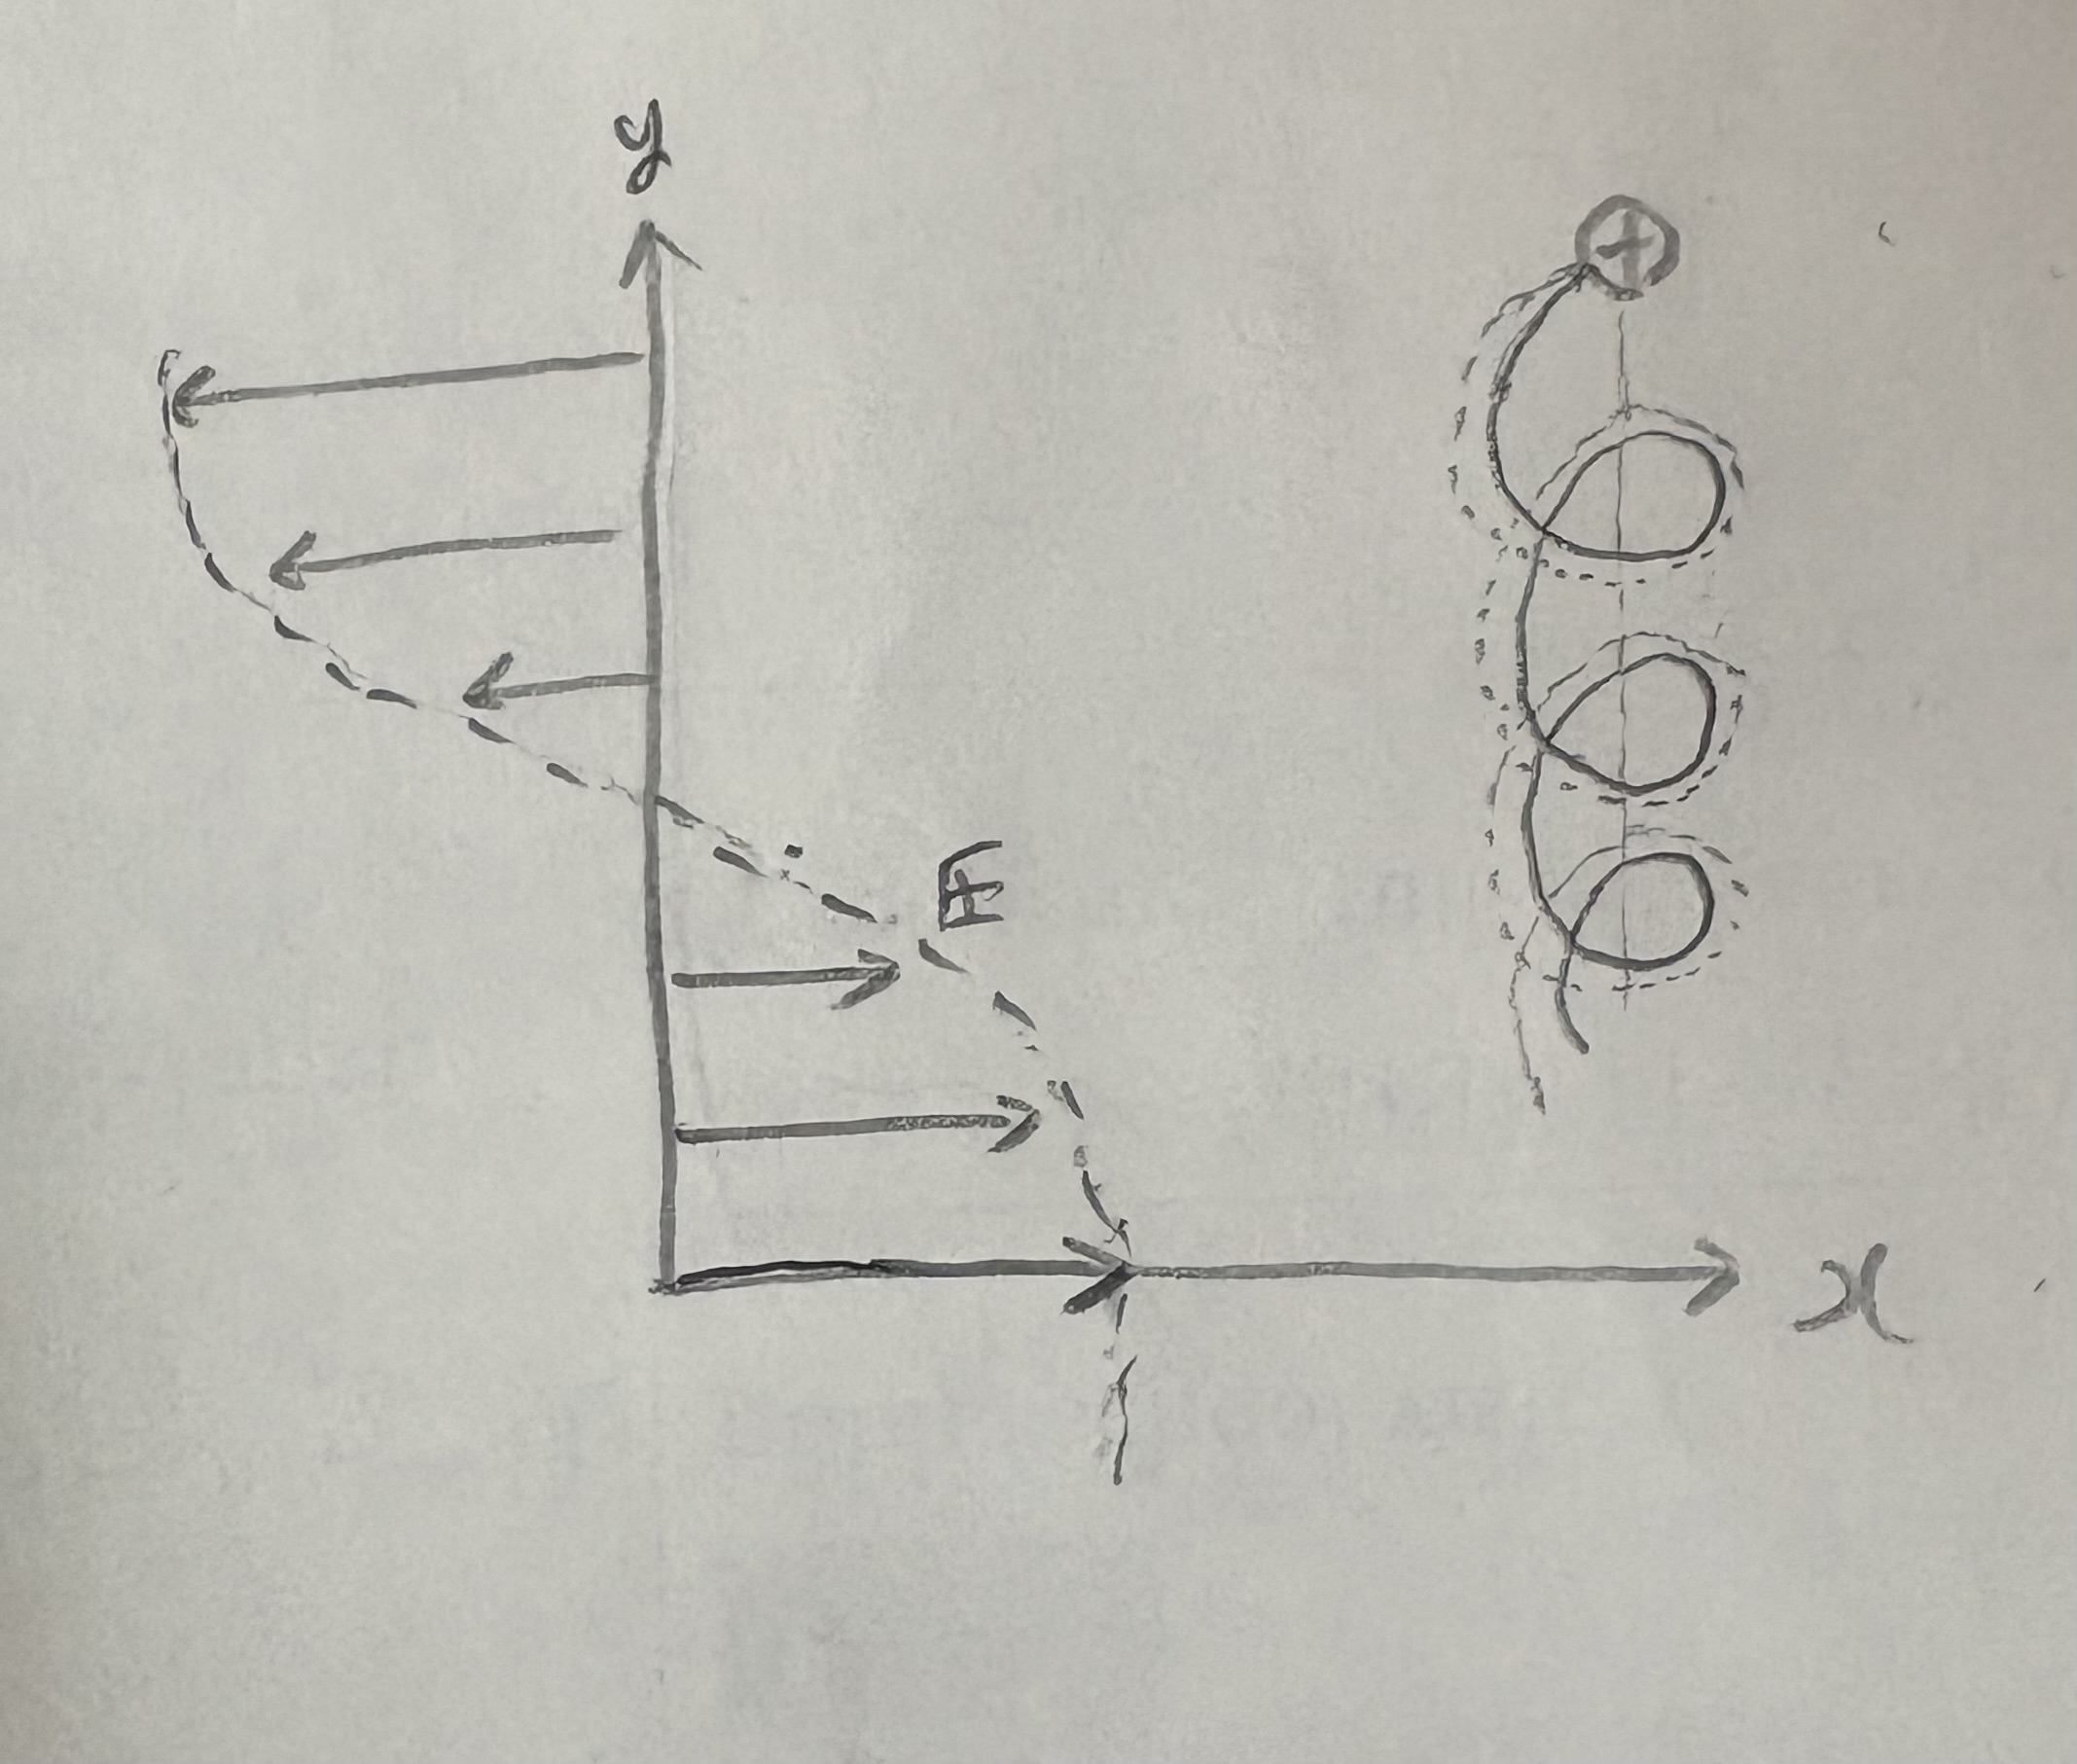
\includegraphics[width=0.5\linewidth]{figg4.jpeg}
  \caption{修正された$\bm{E}\times \bm{B}$ドリフト．点線は一様電場のときの粒子の軌道．粒子は一様電場のときよりも弱い電場中を進むため，Larmor半径はわずかに小さくなる．}
  \label{figg_4}
\end{figure}


\subsection{grad B ドリフト}
図\ref{fig.gradB_drift}のようにz方向の磁場がy方向に応じて密度（大きさ）が増えるとする．
この場合の粒子の軌道は予想できる．上部と下部での磁場の大きさの違いによりLarmor半径が変わり，その差がドリフトを生み出す．（$\bm{E}\times \bm{B}$ドリフトと同じ原理．）

1回転について平均したローレンツ力$\bm{F} = q\bm{v} \times \bm{B}$について考える．$\bar{F_x}$について，図\ref{fig.gradB_drift}からわかるように，下部および上部での回転それぞれで$F_x$はちょうど打ち消し合うため，$\bar{F_x}=0$である．

\begin{figure}[htbp]
  \centering
  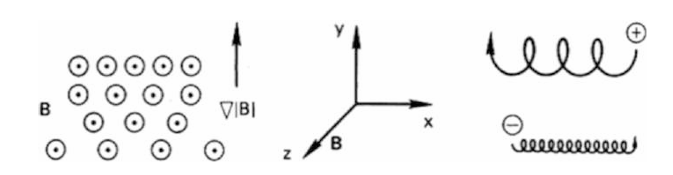
\includegraphics[width=0.7\linewidth]{gradB_drift.png}
  \caption{非一様磁場でのドリフト}
  \label{fig.gradB_drift}
\end{figure}

$\bar{F_y}$は近似的に求めることになるが，ゆがみのない粒子軌道を考えることから出発する．ゆがみのない粒子軌道は一様磁場で

\[
  v_x = v_\perp \cos{\omega_c t}
\]
\[
  y = y_0 \pm \frac{v_\perp}{\omega_c}\cos{\omega_ct}
\]
である．$r_L/L\ll 1$を満たす任意の場所において$\bm{B}$は1次までのテーラー展開で表せる．

\begin{equation}
  \bm{B} = \bm{B}_0 + (\bm{r}\cdot \nabla)\bm{B} + \cdots
\end{equation}
\[
  B_z = B_0 + y(\partial B_z/\partial y) + \cdots
\]
展開点に$x_0=0, y_0=0$を選ぶことで

\begin{equation}
  F_y = -qv_x B_z(y) = -qv_\perp (\cos{\omega_ct})\left[B_0 \pm r_L(\cos{\omega_c t})\frac{\partial B}{\partial y}\right] \label{grad_B_drift}
\end{equation}
\eqref{grad_B_drift}式の第一項は1回転で平均すれば0となる．第二項は$\cos^2{\omega_c t}$の平均が1/2であることから

\begin{equation}
  \bar{F_y} = \mp q v_\perp r_L \frac{1}{2}\frac{\partial B}{\partial y}
\end{equation}
これより，旋回中心のドリフト速度は式\eqref{drift_F}より

\begin{equation}
  \bm{v}_{gc} = \frac{1}{q}\frac{\bm{F} \times \bm{B}}{B^2} = \frac{1}{q} \frac{\bar{F_y}}{|B|}\hat{\bm{x}} = \mp \frac{v_\perp r_L}{B} \frac{1}{2} \frac{\partial B}{\partial y}\hat{\bm{x}}
\end{equation}
これには平均化した力をそのまま式\eqref{drift_F}に使っていいのかといった疑問を抱くかもしれないが，grad B ドリフトよりも旋回運動の方がずっと速いため，平均を考えた1周はドリフトにとっては一瞬であると考えられるので問題はない．
これをより一般的に書くと，$\bm{E}\times \bm{B}$ドリフトと同じ計算で

\begin{equation}
  \boxed{\bm{v}_{\nabla B} = \pm \frac{1}{2}v_\perp r_L \frac{\bm{B}\times \nabla B}{B^2}} \label{df.grad_B_drift}
\end{equation}
この$\bm{v}_{\nabla B}$は\textcolor{red}{grad B ドリフト}と呼ばれる．ここでもドリフトを生じさせる要因は軌道上部と下部でのLarmor半径の差である．
注意すべき点は，$\pm$が表すようにイオンと電子で方向が反対になり，$\bm{B}$に垂直な方向に電流が生じる．

\begin{figure}[H]
  \centering
  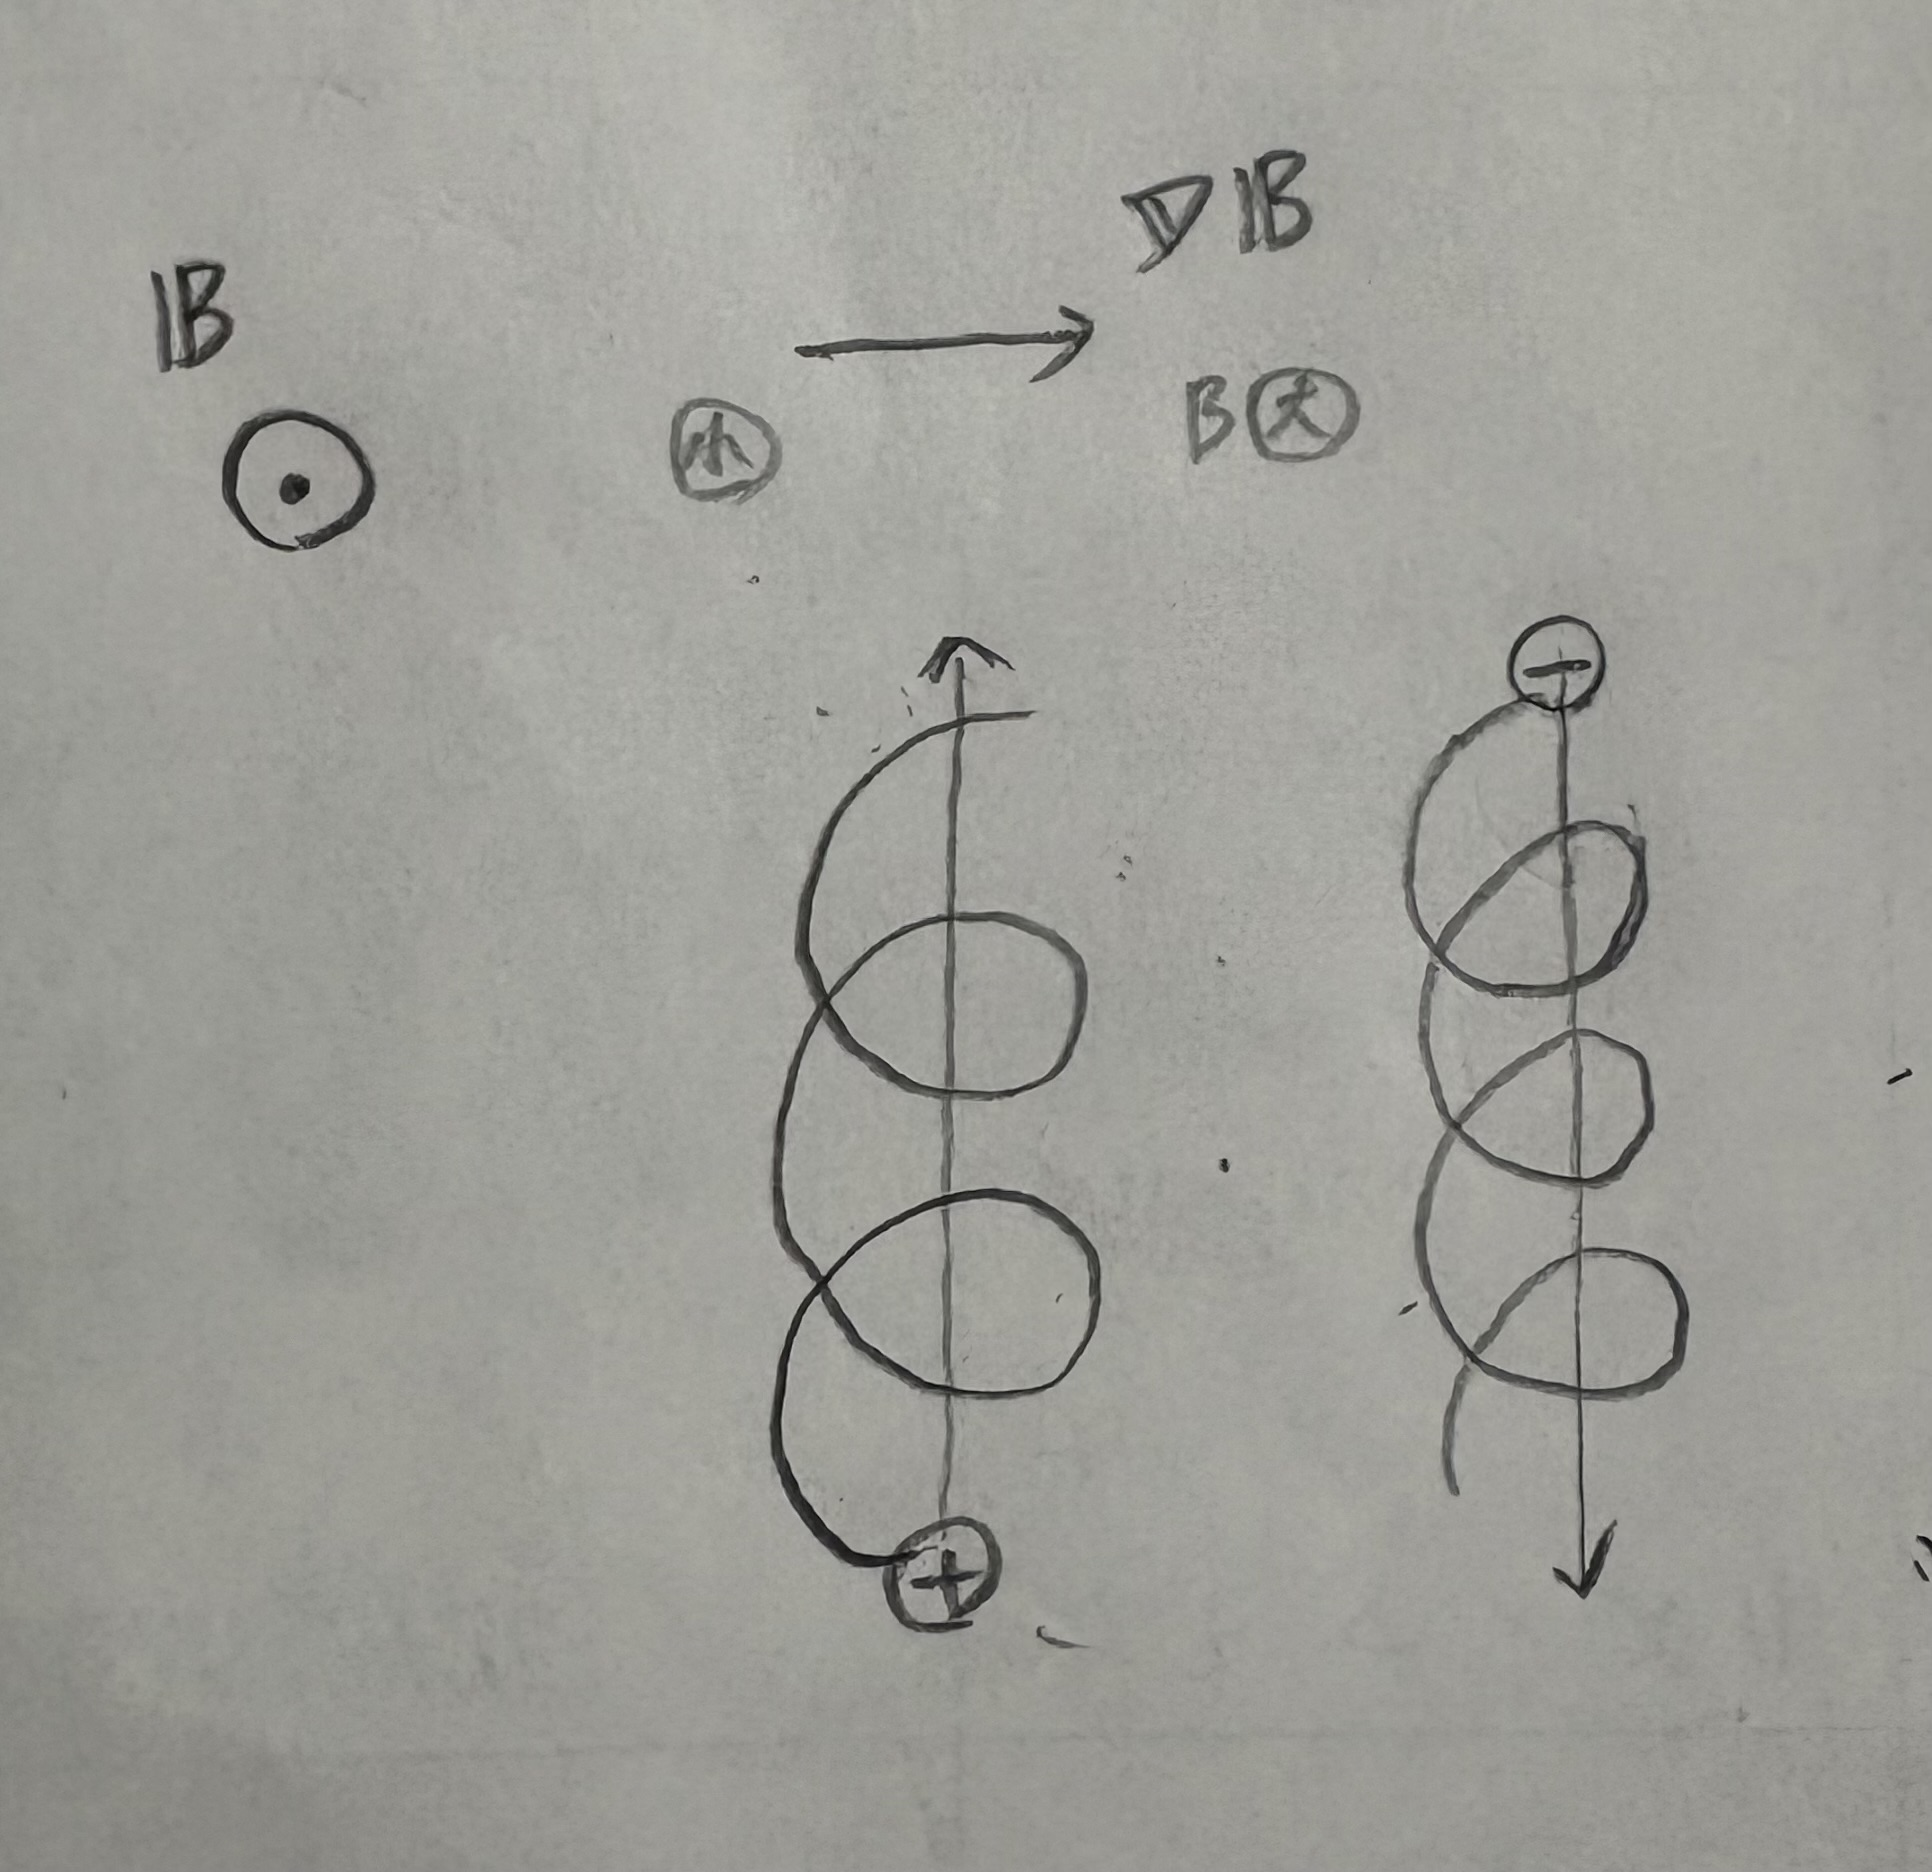
\includegraphics[width=0.5\linewidth]{figg5.jpeg}
  \caption{grad B ドリフトの様子．イオンと電子で方向が反対になる．}
  \label{figg_5}
\end{figure}


\subsection{湾曲ドリフト}
磁力線が一定の曲率半径$R_c$で湾曲しており，|B|は一定である場合を考える（図\refeq{fig.curvature}）．

\begin{figure}[H]
  \centering
  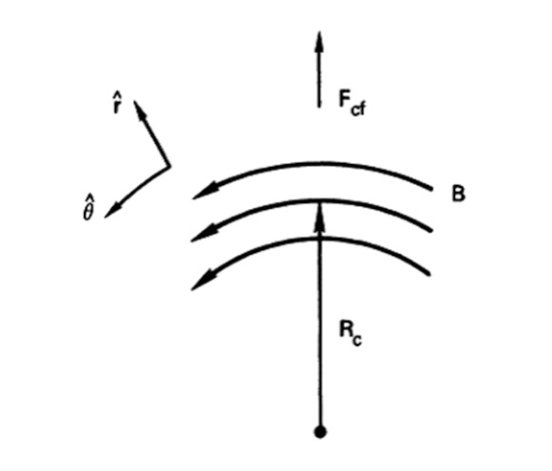
\includegraphics[width=0.5\linewidth]{curvature.png}
  \caption{湾曲磁場}
  \label{fig.curvature}
\end{figure}

粒子が熱運動で磁力線に沿って移動する際に，粒子が受ける遠心力により旋回中心のドリフトが起きる．ランダムな速度の$\bm{B}$方向の2乗平均を$v_\parallel ^2$と表すと，
平均的な遠心力は

\begin{equation}
  \bm{F}_{cf} = \frac{mv_\parallel ^2}{R_c} \hat{\bm{r}} = mv_\parallel ^2 \frac{\bm{R}_c}{R_c ^2}
\end{equation}
これによって起きるドリフト速度は式\eqref{drift_F}より

\begin{equation}
  \boxed{\bm{v}_R = \frac{1}{q}\frac{\bm{F}_{cf} \times \bm{B}}{B^2} = \frac{mv_\parallel ^2 }{qB^2} \frac{\bm{R}_c \times \bm{B}}{R_c ^2}}
\end{equation}
このドリフト$\bm{v}_R$は\textcolor{red}{湾曲ドリフト}と呼ばれる．このドリフトは遠心力が駆動力となっている．湾曲ドリフトが生じる際は磁場が空間変化しているため，必ずgrad B ドリフトもともに生じる．


\subsection{湾曲真空磁場}
上に述べたように，湾曲磁場では，湾曲ドリフトに加えてgrad B ドリフトも生じる．grad B ドリフトを曲率半径方向の|B|の減少を考慮して計算してみる．真空中ではMaxwell方程式より，$\nabla \times \bm{B} = 0$が成り立っている．
図\ref{fig.curvature}の円柱座標において，$\bm{B}$は$\theta$方向の成分のみ，$\nabla B$はr方向の成分のみであるため，$\nabla \times \bm{B}$はz成分のみとなる．
円柱座標系で表されたベクトル場$\bm{A}$の回転$\nabla \times \bm{A}$は
\[
 \nabla \times \bm{A} = \left\{\frac{1}{r}\frac{\partial A_z}{\partial \theta}\right\}\bm{e}_r + \left\{\frac{\partial A_r}{\partial z}-\frac{\partial A_z}{\partial r}\right\}\bm{e}_\theta + \dfrac{1}{r}\left\{\frac{\partial}{\partial r}(rA_\theta) - \frac{\partial A_r}{\partial \theta}\right\}\bm{e}_z
\]
で表されるので

\begin{equation}
  (\nabla \times \bm{B})_z = \frac{1}{r}\frac{\partial}{\partial r} (rB_\theta) = 0 \hspace{2pc} B_\theta \propto \frac{1}{r} \hspace{2pc} \therefore |B| \propto \frac{1}{R_c}
\end{equation}
また，
\[
  \nabla |B| = \frac{d|B|}{dr}\hat{r} \propto -\frac{1}{R_c^2}\hat{r} 
\]
より
\begin{equation}
  \frac{\nabla |B|}{|B|} = -\frac{\bm{R}_c}{R_c ^2}
\end{equation}
これより，\eqref{df.grad_B_drift}式を用いて

\begin{equation}
  \bm{v}_{\nabla B} = \mp \frac{1}{2}\frac{v_\perp r_L}{B^2}\bm{B}\times |B| \frac{\bm{R}_c}{R_c ^2} = \pm \frac{1}{2} \frac{v_\perp ^2}{\omega_c}\frac{\bm{R}_c \times \bm{B}}{R_c ^2B^2} = \frac{1}{2}\frac{m}{q}v_\perp ^2 \frac{\bm{R}_c \times \bm{B}}{R_c ^2 B^2}
\end{equation}
前の$\bm{v}_R$にこれを加えて，真空湾曲磁場中でのドリフトは
\begin{equation}
  \boxed{\bm{v}_R + \bm{v}_{\nabla B} = \frac{m}{q} \frac{\bm{R}_c \times \bm{B}}{R_c ^2 B^2}\left(v_\parallel ^2 + \frac{1}{2}v_\perp ^2\right)}
\end{equation}
となる．

このようなドリフトが加わるのは望ましくない．なぜなら，曲率ドリフト$\bm{v}_R$とgrad B ドリフト$\bm{v}_{\nabla B}$が同じ垂直方向に出て加算されるため，案内中心は一方向に単調にずれていき，
最終的に外に出てしまう．核融合プラズマを閉じ込める目的で磁場をトーラス状にしても閉じ込められないのである．

\begin{figure}[H]
  \centering
  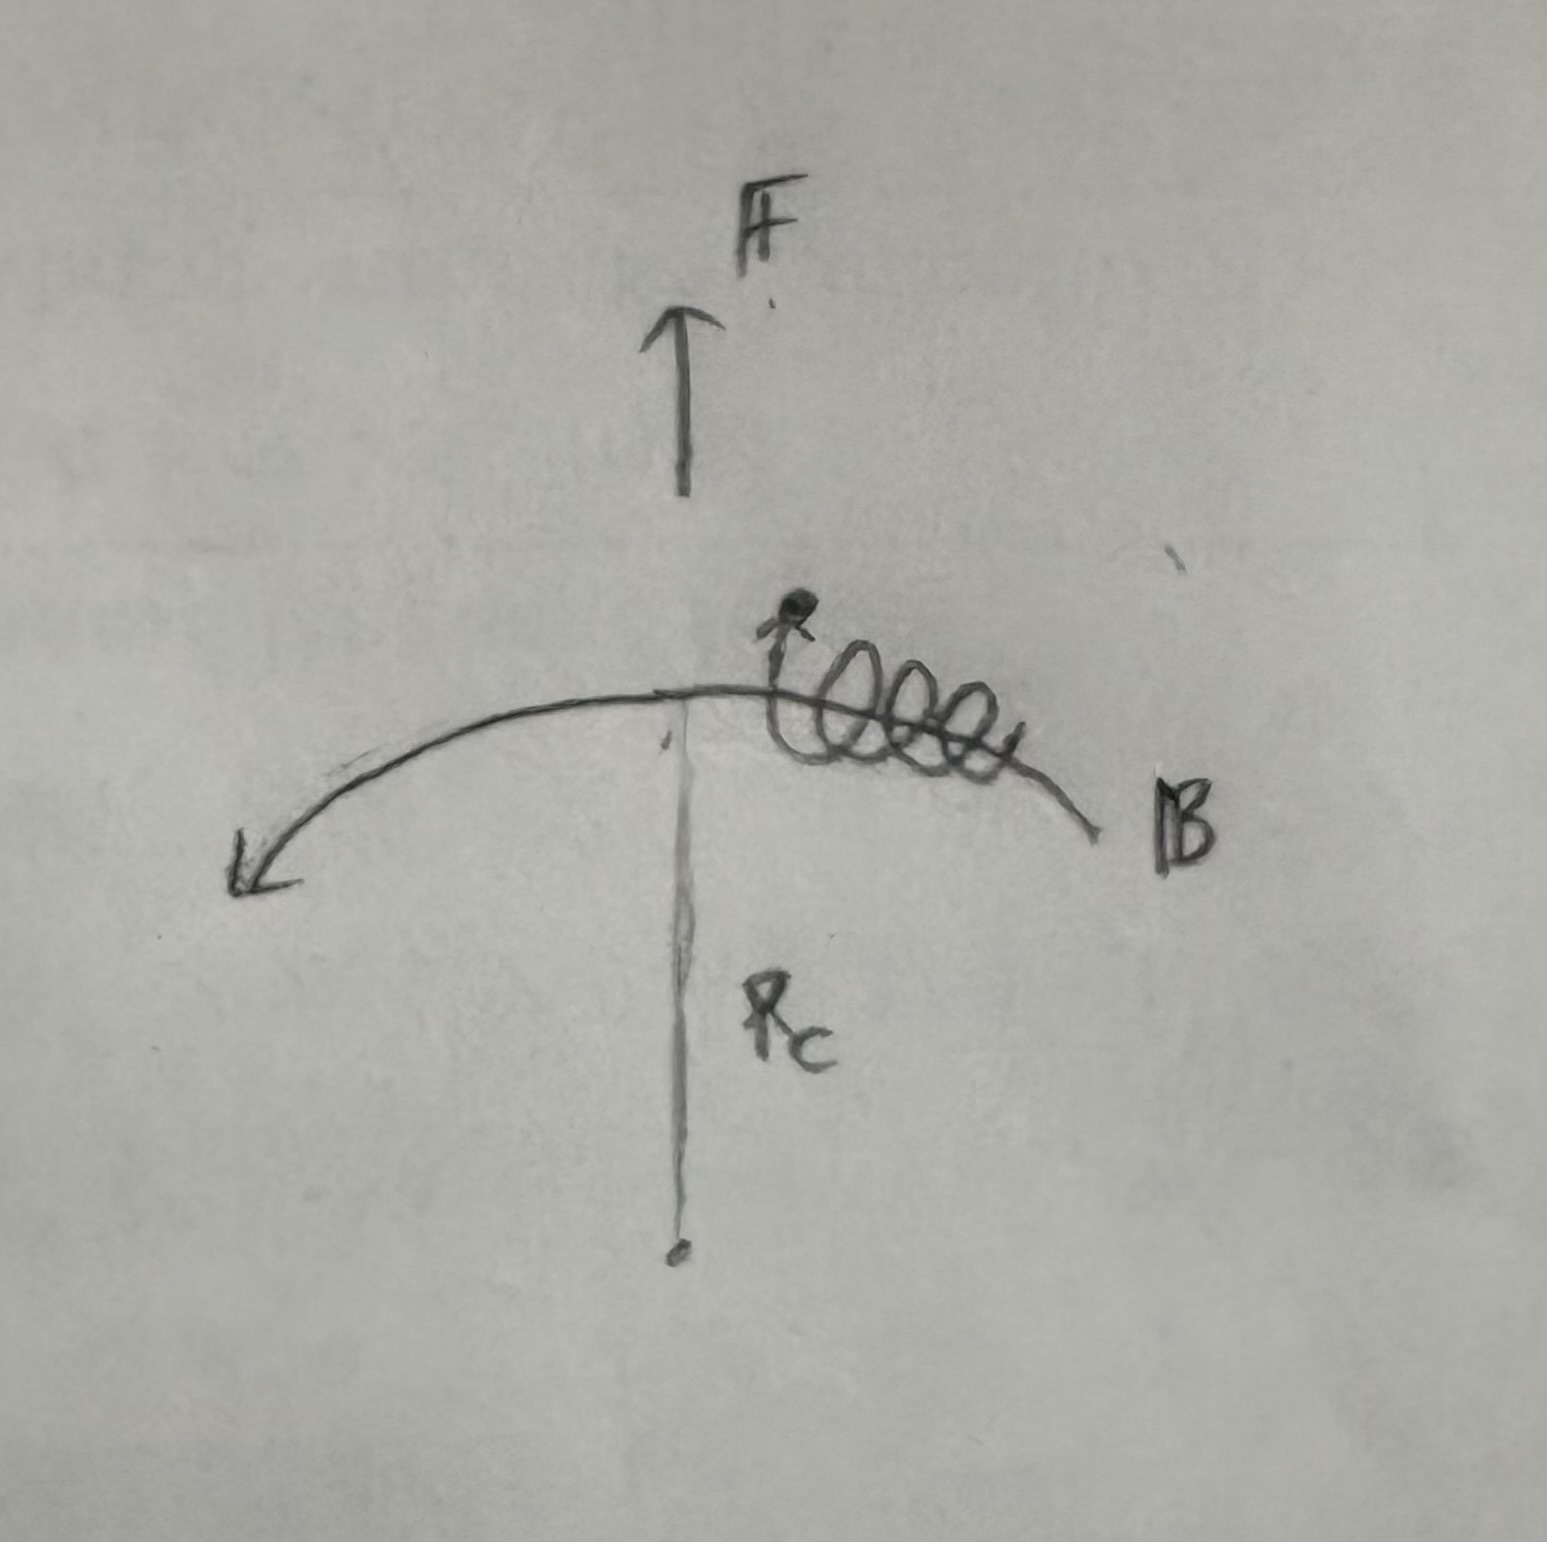
\includegraphics[width=0.5\linewidth]{figg6.jpeg}
  \caption{真空湾曲磁場中でのドリフト}
  \label{figg_6}
\end{figure}


\subsection{分極ドリフト}
$\bm{E}$，$\bm{B}$が空間的には一様であるが，時間的に変化する場合を考える．まず初めに，$\bm{E}$のみが時間に関して正弦的に変化する場合を考える．x軸を$\bm{E}$に沿ってとり

\begin{equation}
  \bm{E} = E_0 e^{i\omega t}\hat{\bm{x}} \label{2.60}
\end{equation}
とする．$\dot{E}_x = i\omega E_x$から，式\eqref{2.50}は次のように書き換えられる．

\begin{equation}
  \ddot{v}_x =-\omega_c ^2\left(v_x \mp \frac{i\omega}{\omega_c}\frac{\tilde{E}_x}{B}\right) \label{2.61}
\end{equation}
ここで，次のような量を定義する：

\begin{align}
  \begin{split}
    \tilde{v}_p &\equiv \pm \frac{i\omega}{\omega_c}\frac{\tilde{E}_x}{B}\\
    \tilde{v}_E &\equiv -\frac{\tilde{E}_x}{B}  
  \end{split}
\end{align}

上付きの$\, \tilde{}\, $は単にドリフトが振動していることを強調するためである．これにより，式\eqref{2.50}，\eqref{2.51}は次のように書き換えられる：

\begin{align}
  \begin{split}
    \ddot{v}_x = -\omega^2_c(v_x - \tilde{v}_p)\\
    \ddot{v}_y = -\omega^2_c(v_y - \tilde{v}_E)
  \end{split} \label{2.63}
\end{align}
この形は式\eqref{base_eq}と同じである．同様の推論から，式\eqref{2.63}の解を

\begin{align}
  \begin{split}
    v_x = v_\perp e^{i\omega_c t} + \tilde{v}_p\\
    v_y = \pm iv_\perp e^{i\omega_c t} + \tilde{v}_E
  \end{split} \label{2.64}
\end{align}
と仮定する．時間に対して2階微分すると

\[
  \ddot{\tilde{v}}_p = \pm \frac{i\omega}{\omega_c}\frac{\ddot{\tilde{E}}_x}{B} = \pm \frac{i \omega}{\omega_c}\frac{1}{B}\cdot (-\omega^2)E_x = -\omega^2 \tilde{v}_p
\]
から

\begin{align}
  \ddot{v}_x &= -\omega^2_c v_\perp e^{i\omega_c t} - \omega^2 \tilde{v}_p = -\omega^2_c(v_\perp e^{i\omega_c t}+\tilde{v}_p)+\omega^2_c \tilde{v}_p -\omega^2\tilde{v}_p \nonumber \\
             &= -\omega^2_c v_x + (\omega^2_c - \omega^2)\tilde{v}_p
\end{align}
$v_y$についても同様に式変形することで

\begin{equation}
  \ddot{v}_y = -\omega^2_c v_y + (\omega^2_c - \omega^2)\tilde{v}_E
\end{equation}
式\eqref{2.63}と比較すると，$\omega^2\, \ll \, \omega^2_c$を満たすとき（$\bm{E}$がゆっくり変化するとき），仮定した解は正しかったことになる．

式\eqref{2.64}は案内中心が2つの成分を持っていることを表している．y成分は，$v_E$が周期$\omega$でゆっくりと振動していることを除けば，通常の$\bm{E}\times\bm{B}$ドリフトである．x成分は$\bm{E}$方向の新しいドリフトであり，\textcolor{red}{分極ドリフト}と呼ばれる．
$i\omega$を$\partial/\partial t$に変えることで，分極ドリフトは次のように表される：

\begin{equation}
  \boxed{\bm{v}_p = \pm\frac{1}{\omega_c B}\frac{d\bm{E}}{dt}} \label{2.66}
\end{equation}

分極ドリフトは「慣性による起動時ドリフト」と理解できる．電場の変化率$d\bm{E}/dt$が大きいほど慣性効果は大きく，磁場が強いほどローレンツ力が速く作用して慣性運動が抑えられるため，ドリフトは小さくなる．
電場の変化がゆるやか（$\omega/\omega_c \ll 1$）であればほとんど無視できる．

\begin{figure}[H]
  \centering
  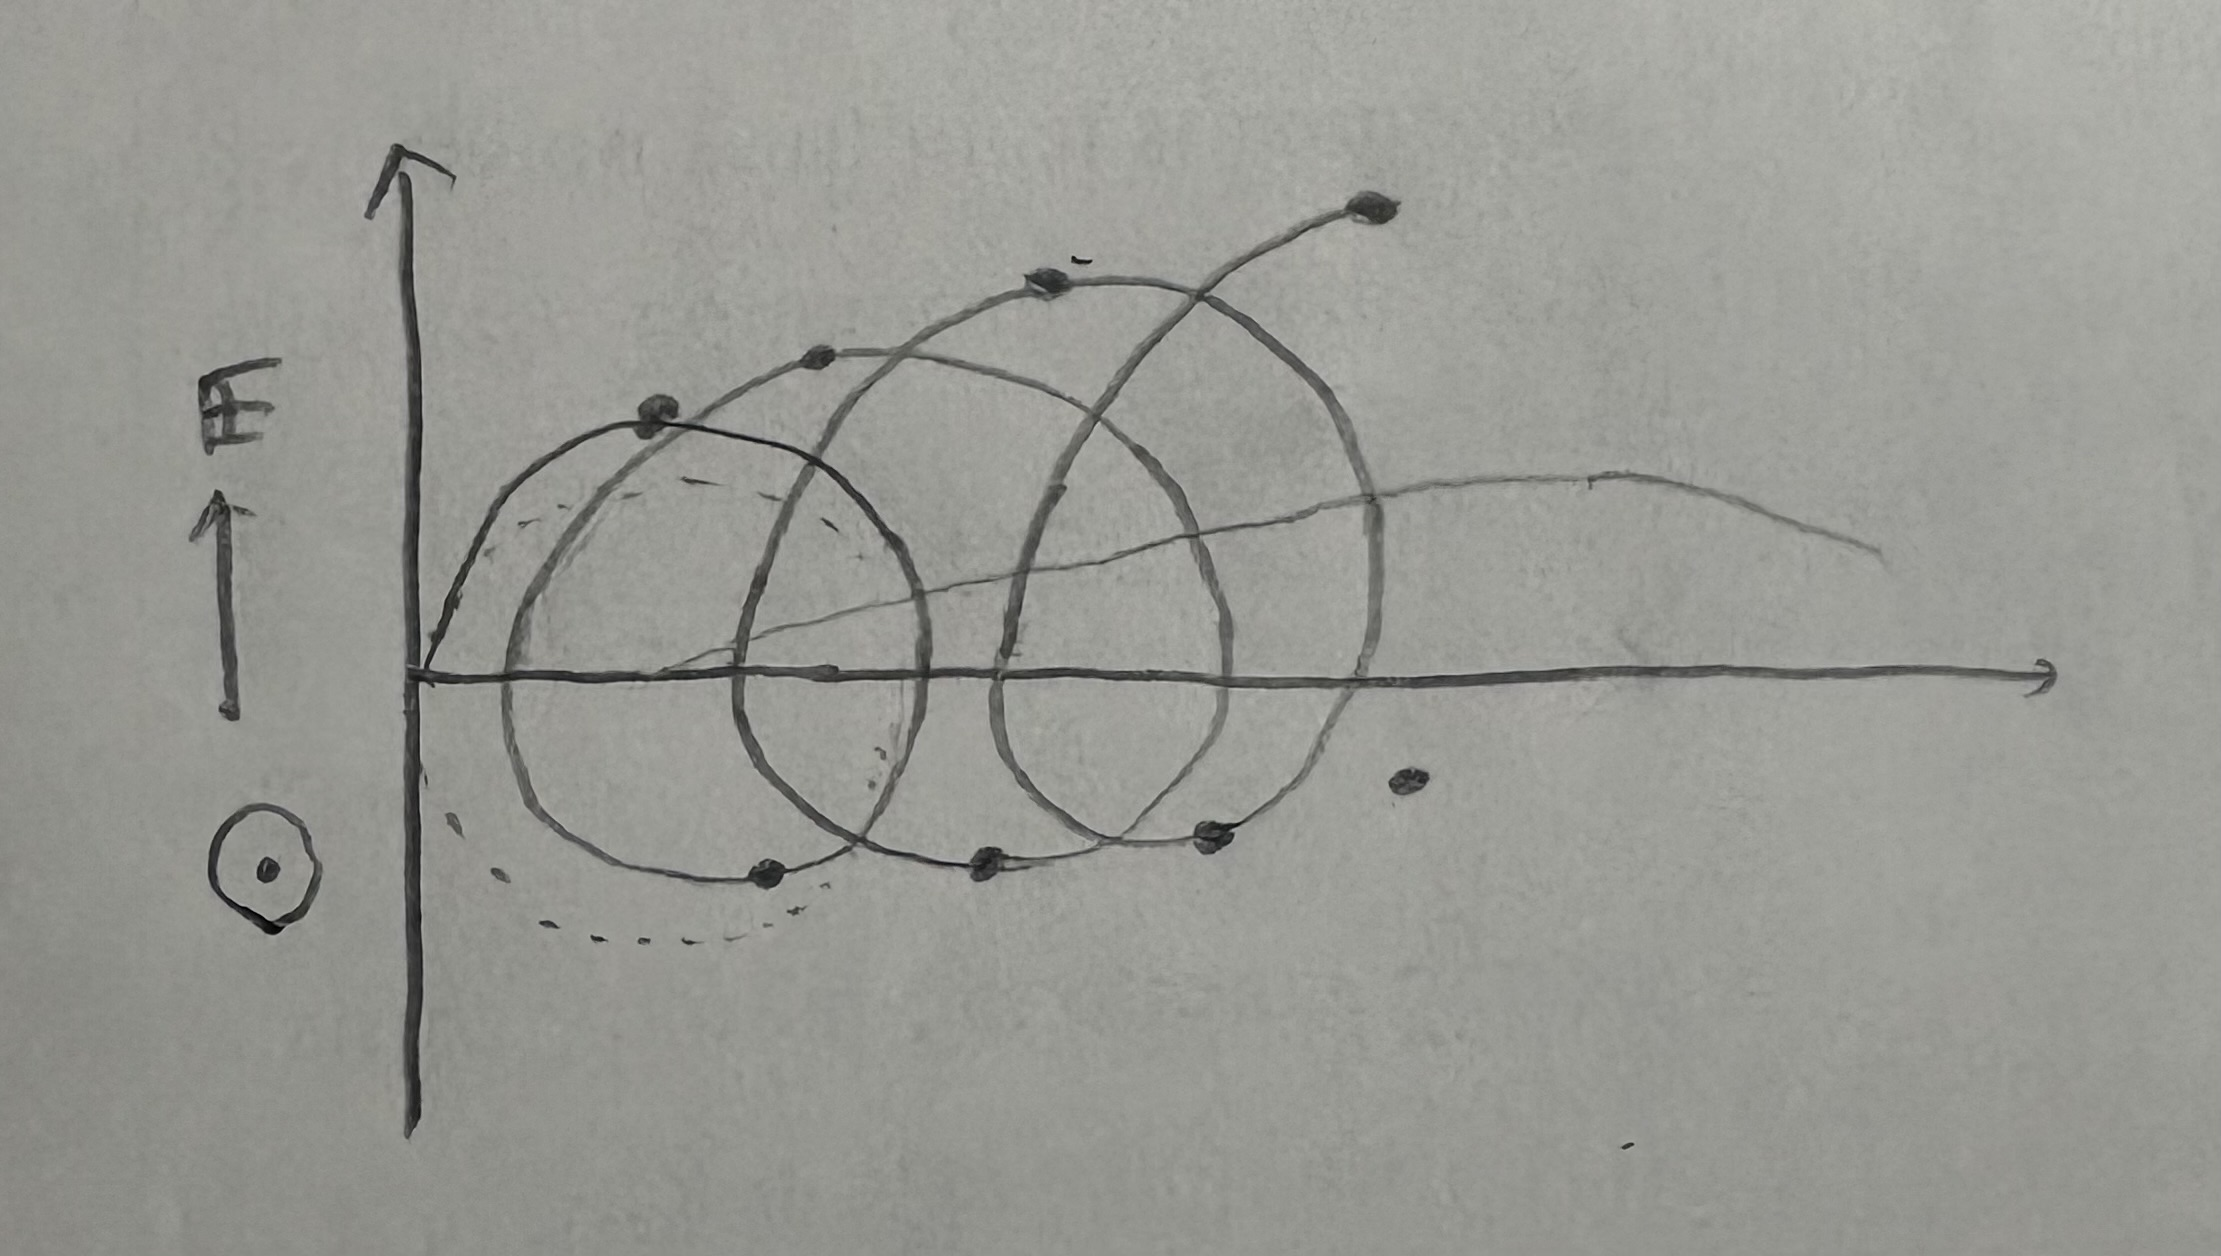
\includegraphics[width=0.5\linewidth]{figg7.jpeg}
  \caption{$E=E_0\cos(\omega t)$で変化する電場中での粒子軌道および旋回中心．旋回中心は$\sin$で変化し，電場から00位相が$\pi/2$遅れている．}
  \label{figg_7}
\end{figure}


\setcounter{section}{3}
\section*{(3)}
\addcontentsline{toc}{section}{(3)}

\subsection*{導出}
磁場のだいたいの方向がz方向で，z方向に強さの変化する磁場を考える．磁場は軸対称であるとすると，$B_\theta = 0$，$\partial/\partial \theta = 0$である（図\refeq{fig.mirror}）．

\begin{figure}[htbp]
  \centering
  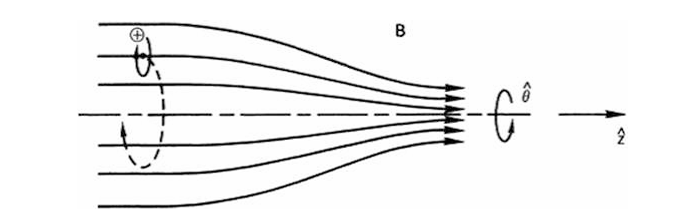
\includegraphics[width=0.7\linewidth]{magnetic_mirror.png}
  \caption{ミラー磁場中での粒子のドリフト}
  \label{fig.mirror}
\end{figure}

$\nabla \cdot \bm{B} = 0$より

\begin{equation}
  \frac{1}{r}\frac{\partial}{\partial r}(rB_r) + \frac{\partial B_z}{\partial z} = 0
\end{equation}
ここで，円柱座標系で表されたベクトル場$\bm{A}$の発散が
\[
  \nabla \cdot \bm{A} = \frac{1}{r}\frac{\partial}{\partial r}(rA_r) + \frac{1}{r}\frac{\partial A_\theta}{\partial \theta} + \frac{\partial A_z}{\partial z}
\]
で表せることを用いた．
$\frac{\partial B_z}{\partial z}$の値が$r=0$で与えられ，$r$とともにあまり大きく変化しないとすると，近似的に

\begin{equation}
  \begin{gathered}
    rB_r = -\int_{0}^{r} r\frac{\partial B_z}{\partial z}dr \simeq -\frac{1}{2}r^2\left[\frac{\partial B_z}{\partial z}\right]_{r=0}\\
    B_r = -\frac{1}{2}r\left[\frac{\partial B_z}{\partial z}\right]_{r=0}    
  \end{gathered} \label{term1234}
\end{equation}
となる．$r$による$|\bm{B}|$の変化はgrad B ドリフトを引き起こすが，$\partial B/\partial \theta = 0$なので，$\nabla B$に$\theta$方向の成分は存在しない．よって，$\bm{B}\times \nabla B$のr方向成分は0であるから，半径方向にはgrad B ドリフトは存在しない．

ローレンツ力の成分は

\begin{align}
  \begin{split}
    F_r     &= q(\underlab{v_\theta B_z}{1}-v_z \cancel{B_\theta})\\
    F_\theta&= q(\underlab{-v_r B_z}{2}+\underlab{v_z B_r}{3})\\
    F_z     &= q(v_r \cancel{B_\theta}-\underlab{v_\theta B_r}{4})
  \end{split}
\end{align}
$B_\theta = 0$より2つの項が消える．➀項と➁項は通常のLarmor運動を引き起こす項である．➂項は軸上では消え，軸から離れたところでは、

\[
  \bm{F} \times \bm{B} = (F_\theta \hat{\theta}) \times (B_r \hat{r}+B_z \hat{z}) = F_\theta B_z \hat{r} - F_\theta B_r \hat{z}
\]
ここで、$B_z \gg B_r$の近似を用いると、
\[
 \bm{F} \times \bm{B} = F_\theta B_z \hat{r} = qv_zB_rB_z\hat{r}
\]
これをドリフトの一般式に代入すると、
\begin{equation}
  \bm{v}_{d} = \frac{\bm{F} \times \bm{B}}{qB^2} = \frac{qv_zB_rB_z}{q(B_z^2+B_r^2)}\hat{r} \simeq v_z \frac{B_r}{B_z}\hat{r} \hspace{2pc} (B_z \gg B_r) \label{v_d,r}
\end{equation}
となり、r方向のドリフトを引き起こすことがわかる。

次に，磁力線に沿う運動の必要条件を求めてみる．磁力線の幾何から
\[
  dr:dz=B_r:B_z \quad \to \quad \frac{dr}{dz} = \frac{B_r}{B_z} 
\]
が成り立つ．これより$r$の変化率は
\begin{equation}
  \frac{dr}{dt} = \frac{dr}{dz}\frac{dz}{dt} = \frac{B_r}{B_z}v_z \label{r_rate}
\end{equation}
となる．式\eqref{v_d,r}と式\eqref{r_rate}を比較すると完全に一致していることがわかる．つまり，ドリフト運動で動くr方向の速度と磁力線のr方向の変化率は一致する．
これはドリフト運動が磁力線に沿って移動していることを表す．長くなったが以上をまとめると，➂項の力が$r$方向のドリフトを引き起こすが，このドリフトは単に旋回中心を磁力線に沿わせるように働く．

結局，注目すべきは➃項である．式\eqref{term1234}より

\begin{equation}
  F_z = \frac{1}{2}qv_\theta r(\partial B_z/\partial z)
\end{equation}
となる．1周にわたって平均をとるが，簡単のため，旋回中心が軸上にあるような粒子を考える．このとき，$v_\theta$は回転の間，一定であり，$q$が$+$のときは時計回り，$-$のときは反時計回りであることを考えると
$v_\theta$は$\mp v_\perp$と書ける．$r=r_L$から平均的な力は

\begin{equation}
  \bar{F_z} = \mp \frac{1}{2}qv_\perp r_L\frac{\partial B_z}{\partial z} = \mp \frac{1}{2}q\frac{v_\perp ^2}{\omega_c}\frac{\partial B_z}{\partial z} = -\frac{1}{2}\frac{mv_\perp ^2}{B}\frac{\partial B_z}{\partial z}
\end{equation}
となる．
回転粒子の磁気モーメントを
\begin{eqbox}{磁気モーメント}
\begin{equation}
 \mu \equiv \dfrac{\frac{1}{2}mv_\perp ^2 }{B}  \label{df.mag_moment}
\end{equation}
\end{eqbox}
で定義すると

\begin{equation}
  \bar{F_z} = -\mu (\partial B_z / \partial z)
\end{equation}
となる．一般的には

\begin{equation}
  \bm{F}_\parallel = -\mu (\partial B /\partial s) = -\mu \nabla_\parallel B \label{F.mag_moment}
\end{equation}
と書かれる．式\eqref{df.mag_moment}の定義が面積$A$，電流$I$の円電流に関する磁気モーメントの定義$\mu= IA$と等価であることに注目してほしい．
1価に帯電したイオンの場合，電荷$e$が1秒間に$\omega_c/2\pi$回回転することにより電流$I$が発生する．$I=e\omega_c/2\pi$，$A=\pi r_L ^2 = \pi v_\perp ^2/\omega_c ^2$より

\[
 \mu = \frac{\pi v_\perp ^2}{\omega_c ^2}\frac{e\omega_c}{2\pi} = \frac{1}{2}\frac{mv_\perp ^2}{B}
\]
となる．

$\mu$が不変量であることを証明しよう．運動方程式の$\bm{B}$に沿った成分は式\eqref{F.mag_moment}を用いて

\begin{equation}
  m\frac{dv_\parallel}{dt} = -\mu \frac{\partial B}{\partial s}
\end{equation}
左辺に$v_\parallel$を，右辺にそれと同値の$ds/dt$をかけると

\begin{equation}
  mv_\parallel \frac{dv_\parallel}{dt} = \frac{d}{dt}\left(\frac{1}{2}mv_\parallel ^2\right) = -\mu \frac{\partial B}{\partial s}\frac{ds}{dt} = -\mu \frac{dB}{dt} \label{time_shift_B}
\end{equation}
ここで，$dB/dt$は粒子から見た$B$の変化であり，$B$自身は時間に対して変化していない．粒子のエネルギーは保存しているはずだから

\begin{equation}
  \frac{d}{dt}\left(\frac{1}{2}mv_\parallel ^2 + \frac{1}{2}mv_\perp ^2\right) = \frac{d}{dt}\left(\frac{1}{2}mv_\parallel ^2 + \mu B\right) = 0
\end{equation}
他にローレンツ力も働いているが仕事をしないので，考えるエネルギーは運動エネルギーのみで良い．式\eqref{time_shift_B}から

\[
 -\mu \frac{dB}{dt} + \frac{d}{dt}(\mu B) = 0
\]
したがって
\begin{equation}
  d\mu/dt = 0
\end{equation}
が証明できた．

$\mu$の不変性は磁気ミラーの原理である．粒子が弱磁場から強磁場へ移動すると，$\mu$一定より$B$の増加に伴い$v_\perp$が増加する．全エネルギー保存のため$v_\parallel$は減少し，十分強い磁場では$v_\parallel=0$となって粒子は反射される．

\begin{figure}[H]
  \centering
  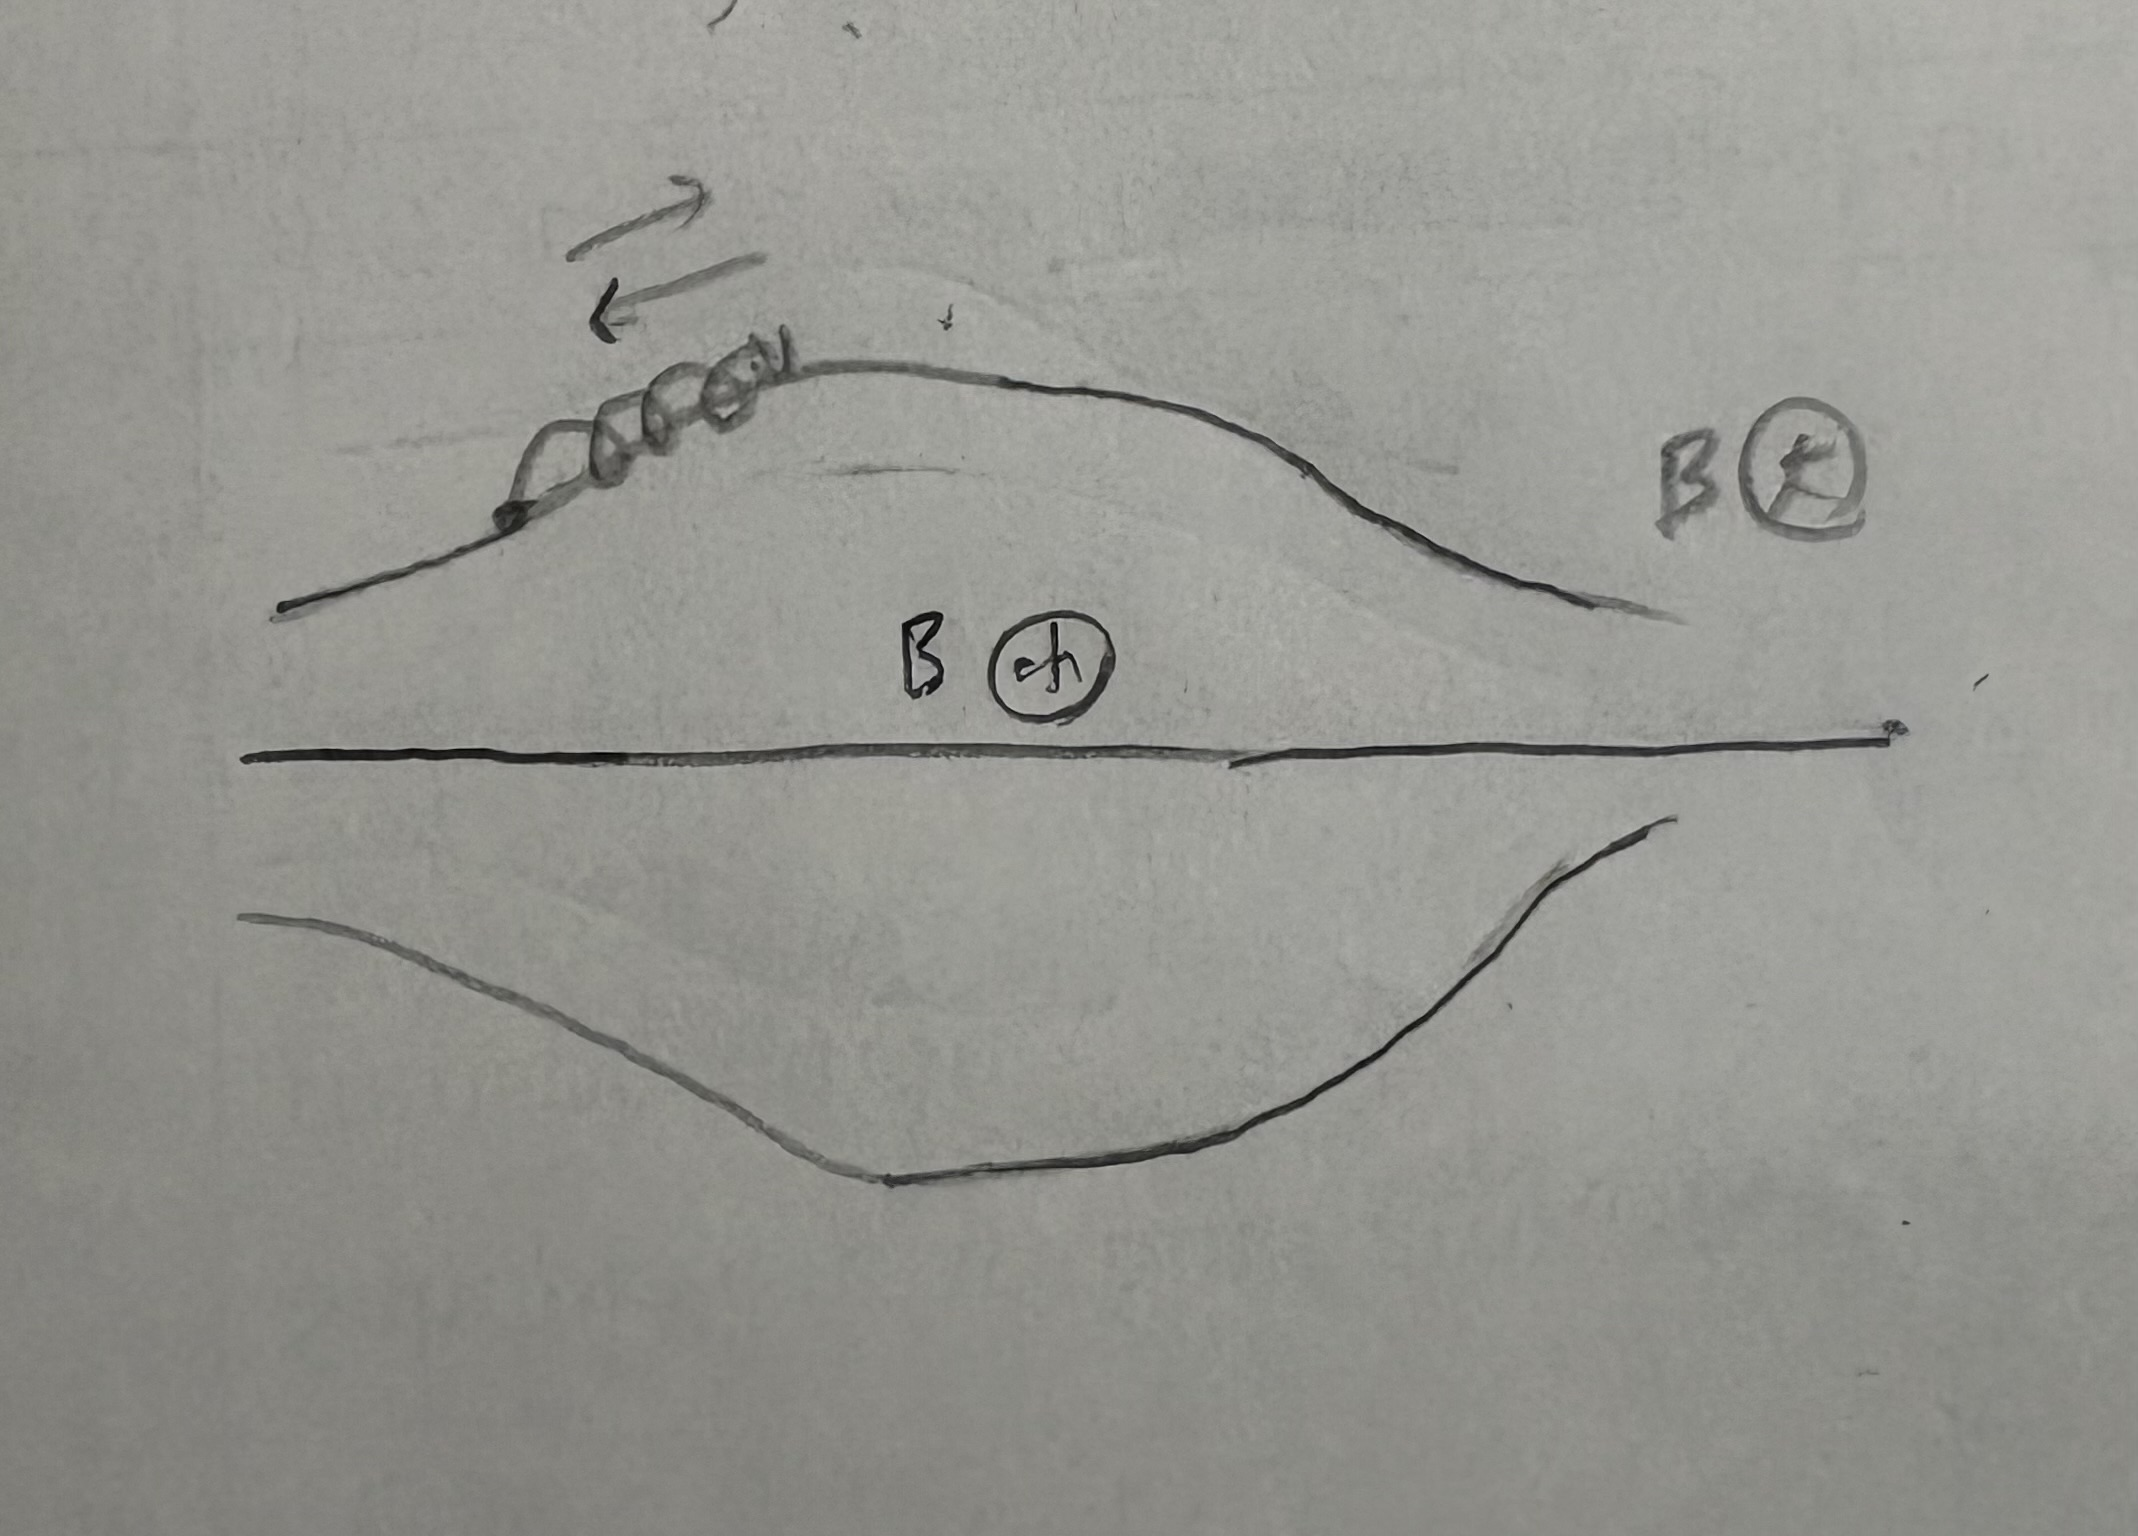
\includegraphics[width=0.5\linewidth]{figg8.jpeg}
  \caption{ミラー磁場中を往復する粒子．}
  \label{figg_8}
\end{figure}


\setcounter{section}{4}
\section*{(4)}
\addcontentsline{toc}{section}{(4)}

\subsection*{導出}
流体要素はするが，粒子はしないというようなドリフトを考える．$\nabla p$項は流体方程式にのみ現れるため，これに関連するドリフトが存在する．運動方程式は，各粒子群につき

\begin{equation}
  mn\left[\underline{\frac{\partial \bm{v}}{\partial t}}_{\text{\large ①}} + \underline{(\bm{v}\cdot\nabla)\bm{v}}_{\text{\large ②}}\right] = qn\left(\bm{E} + \underline{\bm{v}\times\bm{B}}_{\text{\large ③}}\right) - \nabla p \label{3.62}
\end{equation}
となる．ここでは、$\bm{v}_\perp$のみを考える．➂項はLarmor回転運動を表すため，この項に比べると，➀項（$v_\perp$の時間変化）と➁項（$v_\perp$の二次の項）ははるかに小さく，無視できる．したがって，式\eqref{3.62}は
\[
  0 = qn(\bm{E} + \bm{v}\times \bm{B}) - \nabla p
\]
としてもよい．これと$\bm{B}$との外積をとると
\begin{align*}
  0 &= qn[\bm{E}\times \bm{B} + (\bm{v}_\perp \times \bm{B})\times \bm{B}] - \nabla p \times \bm{B}\\
    &= qn[\bm{E}\times \bm{B} + \bm{B}(\bm{v}_\perp \cdot \bm{B}) -\bm{v}_\perp \bm{B}^2] - \nabla p \times \bm{B}
\end{align*}
式変形にベクトル解析の公式$\bm{A}\times (\bm{B}\times \bm{C}) = (\bm{A}\cdot \bm{C})\bm{B} - (\bm{A}\times \bm{B})\bm{C}$を用いた．第2項は0になる．これより

\begin{equation}
  \bm{v}_\perp = \frac{\bm{E}\times \bm{B}}{B^2} - \frac{\nabla p \times \bm{B}}{qnB^2} \equiv \bm{v}_E + \bm{v}_D \label{3.63}
\end{equation}
となる．ここで，
\begin{equation}
  \boxed{\bm{v}_E \equiv \frac{\bm{E}\times \bm{B}}{B^2}} \label{3.64}
\end{equation}
\begin{equation}
  \boxed{\bm{v}_D \equiv -\frac{\nabla p \times \bm{B}}{qnB^2}} \label{3.65}
\end{equation}
と定義した．$\bm{v}_E$はすでに定義した$\bm{E}\times \bm{B}$ドリフトである．$\bm{v}_D$は\textcolor{red}{反磁性ドリフト}と呼ばれる新しいドリフトである．

熱力学の状態方程式（ポアソンの法則）を用いて，$\bm{v}_D$を書き換えることができる．ポアソンの法則は
\begin{equation}
  pV^\gamma = C
\end{equation}
である．物質量を$N$，ボルツマン定数を$N_A$とすると，$N = nV/ N_A$から$V = NN_A/n$を代入すると

\[
  p\left(\frac{NN_A}{n}\right)^\gamma = C
\]
整理して

\begin{equation}
  p = C'n^\gamma \label{3.51}
\end{equation}
を得る．ここで，$C'$は定数，$\gamma$は比熱比$C_p/C_v$である．欲しいのは$\nabla p$であるから，両対数をとり，微分することで

\begin{equation}
  \frac{\nabla p}{p} = \gamma \frac{\nabla n}{n} \label{3.52}
\end{equation}
が得られる．式\eqref{3.52}を用いると，反磁性ドリフトは

\begin{equation}
  \bm{v}_D = \pm \frac{\gamma KT}{eB}\frac{\hat{\bm{z}}\times \nabla n}{n} \label{3.66}
\end{equation}
と書き換えられる．

このプラズマの物理的説明は図\refeq{fig3.5}に示される．ここには，磁場中を旋回しているイオンの軌道が描かれている．左に向かって密度勾配（あるいはそれを生み出す圧力勾配）があるとすると，任意の固定された体積要素を通り抜けるイオンの数は，上方にいくものより下方にいくものの方が多い．
それゆえ，旋回中心は止まっていても$\nabla n$と$\bm{B}$に対して垂直方向に流体のドリフトが生じる．

\begin{figure}[htbp]
  \centering
  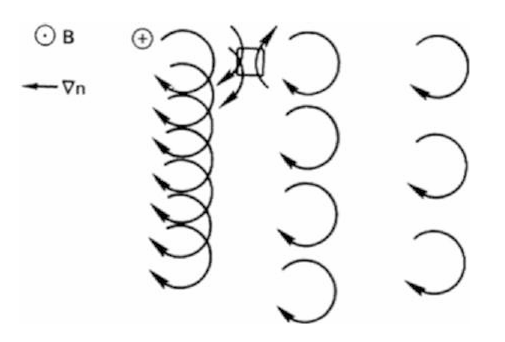
\includegraphics[width=0.6\linewidth]{fig3.5.png}
  \caption{反磁性ドリフトの説明}
  \label{fig3.5}
\end{figure}














\end{document}